\documentclass{article}
\usepackage{tikz, hyperref, comment, amsmath, cleveref, forest, subcaption, listings, xcolor, float}
\usepackage[bottom]{footmisc}
\usepackage[margin=.75in]{geometry}

\renewcommand{\contentsname}{Indice}
\renewcommand{\refname}{Riferimenti}
\renewcommand{\figurename}{Figura}
\renewcommand{\tablename}{Tabella}
\renewcommand{\lstlistingname}{Listato}

\crefformat{section}{\S#2#1#3}
\crefformat{subsection}{\S#2#1#3}
\crefformat{subsubsection}{\S#2#1#3}
\crefformat{figure}{#2Figura~#1#3}
\crefformat{footnote}{#2\footnotemark[#1]#3}
\crefformat{table}{#2Tabella~#1#3}

\crefname{lstlisting}{listato}{listati}
\Crefname{lstlisting}{Listato}{Listati}

\usepackage[listings,skins]{tcolorbox}
\lstdefinelanguage{Toml}{
    comment = [l]{\#},
    keywords = {true, false},
    morestring = [b]{"}
}

\lstdefinelanguage{json}{
    basicstyle=\normalfont\ttfamily,
    numbers=left,
    numberstyle=\scriptsize,
    stepnumber=1,
    numbersep=8pt,
    showstringspaces=false,
    breaklines=true,
    frame=lines,
    backgroundcolor=\color{background},
    literate=
     *{0}{{{\color{numb}0}}}{1}
      {1}{{{\color{numb}1}}}{1}
      {2}{{{\color{numb}2}}}{1}
      {3}{{{\color{numb}3}}}{1}
      {4}{{{\color{numb}4}}}{1}
      {5}{{{\color{numb}5}}}{1}
      {6}{{{\color{numb}6}}}{1}
      {7}{{{\color{numb}7}}}{1}
      {8}{{{\color{numb}8}}}{1}
      {9}{{{\color{numb}9}}}{1}
      {:}{{{\color{punct}{:}}}}{1}
      {,}{{{\color{punct}{,}}}}{1}
      {\{}{{{\color{delim}{\{}}}}{1}
      {\}}{{{\color{delim}{\}}}}}{1}
      {[}{{{\color{delim}{[}}}}{1}
      {]}{{{\color{delim}{]}}}}{1},
}
\lstset{
    tabsize = 2,
    frame = tb,
    breaklines = true,
    numbers = left,
    numbersep = 5pt,
    numberstyle = \color{white!30!black}\scriptsize,
    stepnumber = 1,
    basicstyle = \footnotesize\ttfamily,
    commentstyle={\color{green!50!black}\ttfamily},
    keywordstyle = {\bfseries\color{purple}}, % keywords
    keywordstyle = [2]{\itshape\color{blue}}, % traits
    keywordstyle = [3]{\color{blue}}, % primitive types
    keywordstyle = [4]{\color{blue}}, % type and value ctors
    keywordstyle = [5]{\color{purple!50!blue}}, % macros
    stringstyle = \color{green!45!blue},
    aboveskip = \baselineskip,
    showstringspaces = false
}
 \lstdefinelanguage{docker}{
  keywords={FROM, RUN, COPY, ADD, ENTRYPOINT, CMD,  ENV, ARG, WORKDIR, EXPOSE, LABEL, USER, VOLUME, STOPSIGNAL, ONBUILD, MAINTAINER, HEALTHCHECK},
  keywordstyle=\color{blue}\bfseries,
  identifierstyle=\color{black},
  sensitive=false,
  comment=[l]{\#},
  commentstyle=\color{purple}\ttfamily,
  stringstyle=\color{red}\ttfamily,
  morestring=[b]',
  morestring=[b]"
}
\lstdefinelanguage{Ini}
{
    basicstyle=\ttfamily\small,
    columns=fullflexible,
    morecomment=[s][\color{Orchid}\bfseries]{[}{]},
    morecomment=[l]{\#},
    morecomment=[l]{;},
    commentstyle=\color{gray}\ttfamily,
    morekeywords={},
    otherkeywords={=,:},
    keywordstyle={\color{green}\bfseries}
}

\title{Sistemi Embedded}

\author{Giuseppe Capasso}

\begin{document}
\begin{titlepage}
  \thispagestyle{empty}
  \raggedright % Allinea a sinistra

  \begin{tikzpicture}
    \node[anchor=south west] at (4,0) {
\includegraphics[scale=0.75]{figures/unina-logo-1.png}};
    \node[anchor=south west] at (0,1.5) {
\includegraphics{figures/unina-logo-2.png}};
    \node[anchor=south west] at (0,0.5) {\textsf{Scuola Politecnica e delle Scienze di Base}};
    \node[anchor=south west] at (0,0) {\textsf{Corso di Laurea Magistrale in Ingegneria Informatica}};
  \end{tikzpicture}

  \vfill

  {\textbf{\textit{\LARGE Strumenti per il confidential computing}}}
  \\[2cm]

  {\textbf{\textit{\Large Sistemi Embedded}}}
  \\[1cm]
  {\large Anno Accademico 2023/2024}

  \vfill

  \begin{table}[h]
    \textbf{Giuseppe Capasso matr. M63001498}
  \end{table}

\end{titlepage}

\thispagestyle{empty}
\tableofcontents

\newpage
\thispagestyle{empty}

\section{Confidential computing}
\subsection{Trusted Execution Environment (TEE)}
I Trusted Execution Environment realizzano una forma di isolamento dei processi e delle applicazioni in hardware per rendere sistemi resistenti ad attacchi fisici e \textit{side-channel}. I TEE sono pensati per essere utilizzati dai sistemi operativi (o hypervisor) in maniera alternativa a TPM e HSM. Ogni azienda propone una propria implementazione dei TEE che può andare dalla protezione di applicazioni in spazio utente (come Intel-SGX) a macchine virtuali sicure come (AMD-SEV e Intel TDX).  In questo senso, ogni implementazione fa riferimento ad un \textit{threat model} differente e può includere diversi elementi nella \textbf{\textit{Trusted Computing Base} (TCB)}. La \cref{tab:tee-implementations} riporta una panoramica delle princiapli tecnologie commerciali ed è tratta da \cite{Jauernig2020}. I $2$ approcci principali (\textit{user-space isolation} e \textit{VM isolation}) sono illustrati in \cref{fig:tee-implementations} (tratta da \cite{Jauernig2020}) in cui viene mostrata anche la soluzione \textbf{\textit{Sanctum}} sviluppata per Risc-V.

\begin{figure}[h]
  \begin{center}
    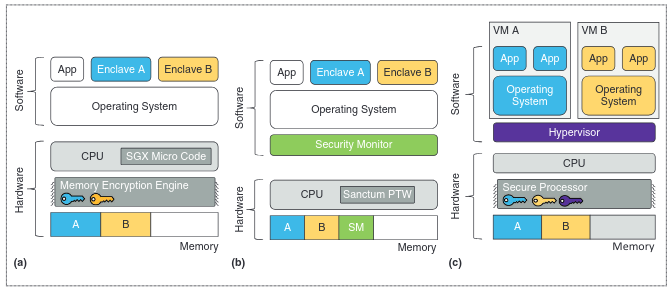
\includegraphics[width=0.95\textwidth]{figures/ch1/tee-implementations.png}
  \end{center}
  \caption{Implementazione TEE in diverse architetture. (a) Intel SGX. (b) Risc-V Sanctum. (c) AMD SEV}\label{fig:tee-implementations}
\end{figure}

\begin{table}
\centering
\begin{tabular}{|p{3cm}|p{3cm}|p{3cm}|p{3cm}|}
\hline
\textbf{} & \textbf{Intel SGX} & \textbf{AMD SEV} & \textbf{ARM TrustZone} \\ \hline
\textbf{Target devices} & Client PCs & Servers & Mobile devices  \\ \hline
\textbf{Trust anchor} & CPU hardware e microcode & Platform security processor & TZ hardware e ARM trusted firmware \\ \hline
\textbf{Cache side-channel protection} & No  & No  & No \\ \hline
\textbf{Multiple security domains} & Si & Si & No \\ \hline
\textbf{Security peripherals} & No & No & Si \\ \hline
\end{tabular}
\caption{Confronto tra Intel SGX, AMD SEV e ARM TrustZone}
\label{tab:tee-implementations}
\end{table}

\subsection{Intel Software Guards Extentions (SGX)}
Intel SGX è la prima forma di confidential computing proposta da Intel con supporto hardware. Lo scopo principale di SGX è quello di estendere l'ISA mettendo a disposzione delle istruzioni riservate per gestire applicazioni confidenziali. In un'applicazione trusted, sia dati che istruzioni non lasciano la CPU in chiaro assicurando tre proprietà:
\begin{itemize}
  \item Confidenzialità: un'altra applicazione non può leggere le istruzioni e i dati di un'applicazione trusted;
  \item Integrità: sia all'avvio che durante l'esecuzione dell'applicazione viene effettuato un controllo crittografico dello spazio di memoria. 
  \item Attestazione: le applicazioni devono poter dimostrare la loro \textbf{\textit{trustworthiness}} sia ad altre applicazioni (\textbf{\textit{local attestation}}) che a sistemi remoti (\textbf{\textit{remote attestation}});
\end{itemize}

SGX aggiunge all'ISA dell'architettura classica $18$ istruzioni con le quali si può creare una regione confidenziale, eseguire il processo di attestazione e verificare l'integrità dell'applicazione. 
SGX prevede un threat model in cui sono considerati trusted solo la CPU e il codice in esecuzione nell'enclave assumendo che un attore malevolo possa prendere effettuare sia attacchi hardware (eg. \textbf{\textit{cold boot}}) che al livello OS (eg. \textbf{\textit{ROP}}).

\subsubsection{Enclave}\label{sec:enclave}
L'\textbf{\textit{enclave}}\cite{Costan2016} è la prima astrazione fornita da SGX e definisce un perimetro di sicurezza all'interno dello spazio di indirizzamento virtuale. La memoria all'interno dell'enclave è cifrata e accessibile solo dall'interno dell'enclave stessa. La memoria viene cifrata con un \textbf{MEE} (\textit{Memory Encryption Engine}) la cui implementazione non è stata discussa ufficialmente.

Codice, dati e metadati di un'enclave vengono gestite da SGX in un'area riservata della DRAM detta \textbf{PRM} (\textit{Processor Reserved Memory}) che contiene la \textbf{EPC} (\textit{Enclave Page Cache}) a cui si accede solo attraverso le istruzioni SGX. La EPC ha una dimensione di $128/256 MB$ e può essere vista come una \textit{cache L3}, ma non impone alcun limite alla dimensione delle enclave visto che è supportato il processo di \textit{eviction}. Il compito di gestire la tabella delle pagine è affidato al sistema operativo o hypervisor. Dato che il gestore della memoria non è parte della TCB, SGX controlla le operazioni effettuate dal gestore della memoria attraverso la \textbf{EPCM} (\textit{Enclave Page Cache Map}).

Un'applicazione trusted deve creare un'enclave con l'istruzione $ECREATE$. SGX assegna per ogni enclave una \textbf{SECS} (\textit{SGX Enclave Control Structure}) in cui vengono conservati tutti i metadata per enclave. In particolare, i metadata sono memorizzati sottoforma di \textbf{attributi}.

Alla creazione, viene allocata una SECS insieme alla EPC. Con l'istruzione $EADD$ vengono caricati codice e dati dell'applicazione: nello specifico vengono copiate pagine dalla parte non trusted del sistema a quella dell'enclave con un controllo validità.
Per essere eseguita, l'enclave deve ottenere un \textbf{EINIT Token Structure}. Questo token viene fornito da un'enclave privilegiata detta \textbf{(LE)} \textit{Launch Enclave} fornita da Intel e firmata con una chiave speciale all'interno dell'architettura SGX. Solo la \textbf{LE} può chiamare la $EINIT$ che può impostare l'attributo \textbf{INIT} a $1$. La terminazione viene fatta con $EREMOVE$ che dealloca la EPC e la EPCM.

Quando un'enclave entra in esecuzione il processore opera in \textbf{enclave mode} con la quale riceve i privilegi di accedere alla EPC. Per poter transitare in enclave mode, il processore deve eseguire una $EENTER$ e per lasciare la modalità esegue una $EEXIT$. $EENTER$ non effettua un cambio di privilegio (si esegue sempre a \textbf{ring 3}), ma effettua un salto memorizzando il \textbf{RIP} (\textit{Return Instruction Pointer}). $EENTER$ è un'operazione sincrona. $EEXIT$ può essere eseguita solo da un processore in enclave mode ed effettua un salto al RIP memorizzato durante il $EENTER$ in maniera sincrona. Nel caso in cui ci sia un'eccezione, l'uscita avviene in maniera asincrona con $AEX$ (\textit{Asynchronous Enclave Exit}).

\paragraph{Limiti di SGX}
Intel SGX, pur offrendo un elevato livello di sicurezza, presenta alcune limitazioni intrinseche che devono essere considerate durante lo sviluppo di applicazioni. Queste limitazioni derivano principalmente dal design dell'architettura e dalle restrizioni imposte per mantenere l'integrità e la sicurezza dell'enclave. Di seguito sono elencate alcune delle principali limitazioni di SGX:

\begin{itemize}
  \item \textbf{Limitazioni di memoria}: la dimensione della \textit{Enclave Page Cache} (EPC) è limitata a 128/256 MB, il che può rappresentare un vincolo significativo per applicazioni che richiedono grandi quantità di memoria. Sebbene SGX supporti il processo di \textit{eviction}, questo può introdurre overhead prestazionale;
  \item \textbf{Assenza di protezione contro attacchi side-channel}: SGX non fornisce protezione contro attacchi side-channel basati su cache, timing, o power analysis. Questi attacchi possono potenzialmente rivelare informazioni sensibili anche se l'enclave è isolata;
  \item \textbf{Limitazioni nelle operazioni di I/O}: le enclavi SGX non possono eseguire direttamente operazioni di I/O. Tutte le operazioni di I/O devono essere delegate al sistema operativo host, il che richiede un'uscita dall'enclave (\textit{ocall});
\end{itemize}

\paragraph{Comunicazione con mondo esterno} Date le limitazioni, SGX fornisce un meccanismo per interagire con l'input output attraverso le \textbf{\textit{Enclave Call} (ECALL)} (per eseguire una funzione in ambiente sicuro) e le \textbf{\textit{Out Call} (OCALL)} (esegue una funzione in spazio non \textit{trusted}). Queste due tipologie di operazioni non comportano un cambio di privilegio strettamente, ma, ad esempio una \textit{OCALL} consente di eseguire una system call (o di interfacciarsi con l'I/O). Questa sequenza di operazioni è una delle principali fonti di degradazione delle prestazioni in applicazioni I/O bound in SGX perchè il sistema spende molto tempo nella fase EENTER  e EEXIT, come illustrato in \cref{fig:enclave-lifecycle}

\begin{figure}
  \begin{center}
    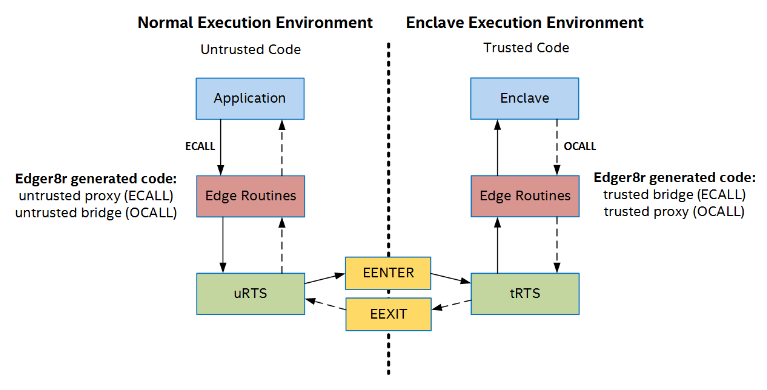
\includegraphics[width=.85\textwidth]{figures/ch1/enclave-lifecycle.png}
  \end{center}
  \caption{Ciclo di vita di un'enclave}\label{fig:enclave-lifecycle}
\end{figure}

\subsubsection{Attestazione}
L'attestazione è un processo fondamentale nel confidential computing che consente di verificare l'integrità e l'affidabilità di un'applicazione o di un ambiente di esecuzione. Questo processo permette a un'entità di dimostrare a un'altra entità che il proprio stato è sicuro e che non è stato compromesso.Esistono due tipi principali di attestazione: 
\begin{itemize}
  \item locale: avviene tra componenti all'interno dello stesso sistema;
  \item remota: coinvolge la verifica da parte di un'entità esterna.
\end{itemize}

In SGX, l'attestazione viene creata da un'altra enclave privilegiata detta \textbf{QE} (\textit{Quoting Enclave}) gestita da Intel che può accedere alla chiave per firmare l'attestazione. Prima di procedere con l'attestazione remota, bisogna creare un canale di comunicazione sicuro con la quoting enclave e, pertanto, è previsto un sistema di attestazione locale. 

Una volta creato, l'enclave genera un report, popolato i campi con la relativa SECS, con l'istruzione $EREPORT$, lo firma con una chiave scambiata con la $QE$ e allega anche un MAC per il controllo dell'integrità.

È bene notare che la chiave con cui viene firmato il report dalla QE non è presente all'interno di SGX all'uscita dalla fabbrica, ma viene generata utilizzando un \textit{Provisioning Enclave} con l'istruzione $EGETKEY$ il cui processo non è documentato, ma ha come input valori accessibili solo all'interno del processore come il \textbf{\textit{Secure Version Number (SVN)}}.

L'attestazione può essere fatta con due procedimenti: EPID (\cref{fig:ra-epid}, utilizzata da remoto) o con DCAP (\cref{fig:ra-dcap}). Le due figure sono molto simili, ma con DCAP il servizio Intel viene contattato solo una volta dal \textit{Provisioning Enclave} e non ogni volta come in EPID. Come spiegato in \cref{sec:dcap-infrastructure-configuration}, l'attestazione EPID è deprecata e quindi non sarà approfondita.

\begin{figure}[h]
\centering
\begin{subfigure}{.5\textwidth}
  \centering
  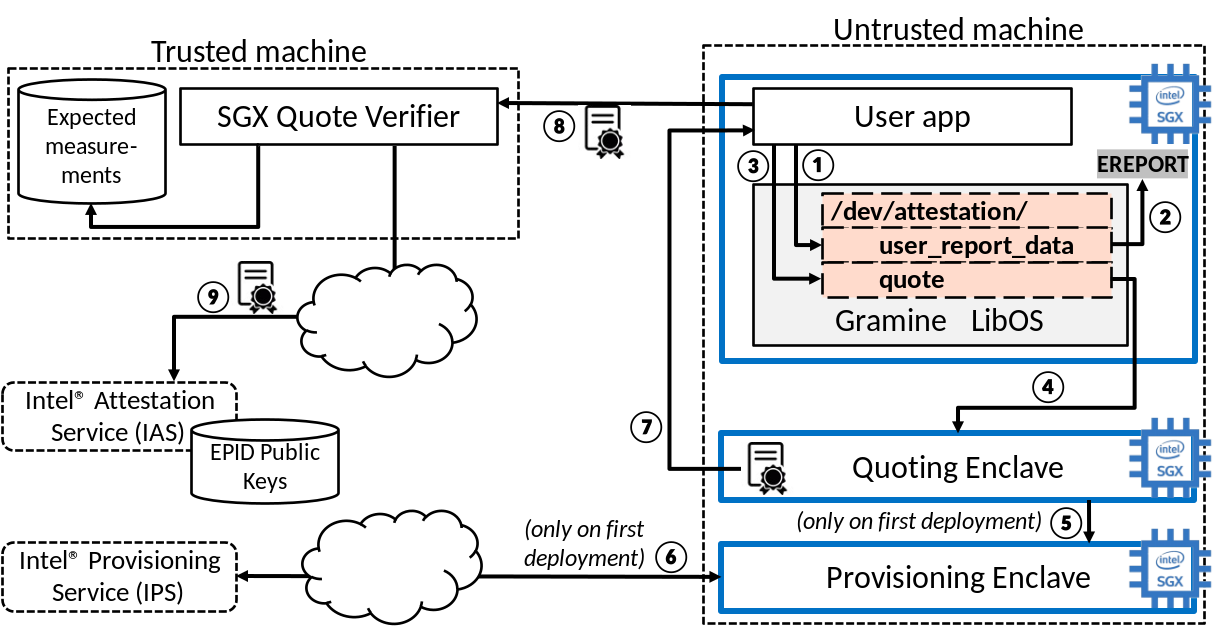
\includegraphics[width=.95\textwidth]{figures/ch1/ra-sgx-epid.png}
  \caption{Attestazione remota con EPID}\label{fig:ra-epid}
\end{subfigure}%
\begin{subfigure}{.5\textwidth}
  \centering
    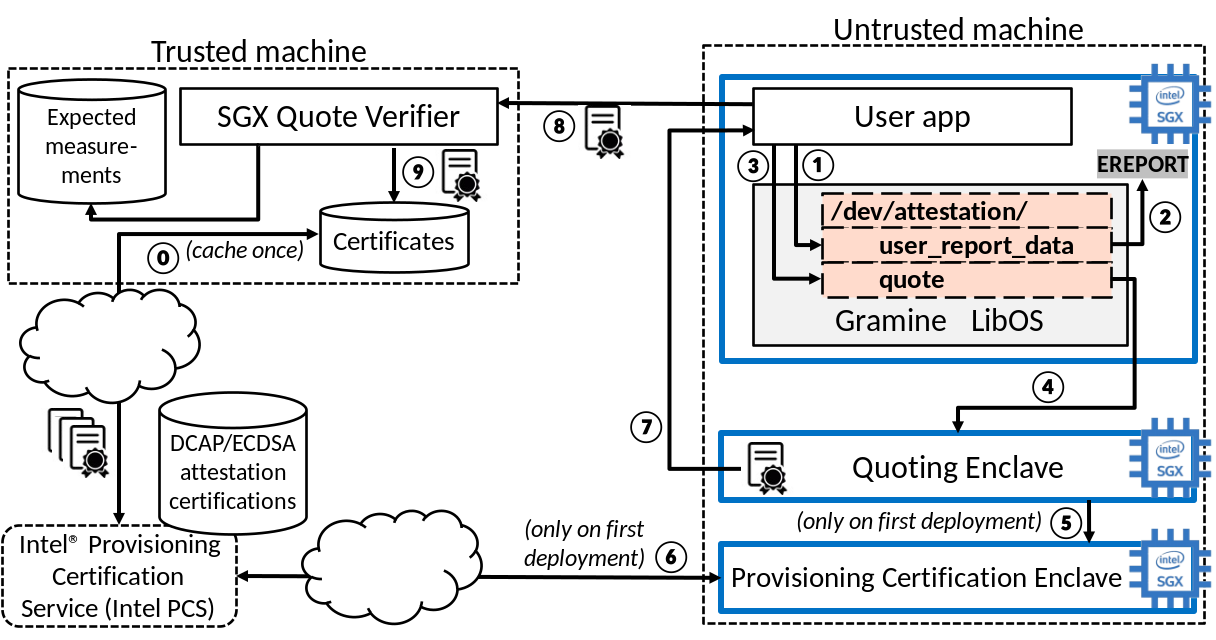
\includegraphics[width=.95\textwidth]{figures/ch1/ra-sgx-dcap.png}
  \caption{Attestazione locale con DCAP}\label{fig:ra-dcap}
\end{subfigure}
\caption{Confronto tra attestazione remota con EPID e DCAP}
\end{figure}

\subsubsection{SGX2}
L'architettura descritta in \cref{sec:enclave} è implmentata completamente in SGX1. In \cite{10.1145/2948618.2954331}, è mostrata un'estensione della versione base di SGX a cui ci si riferisce come SGX2. Il componente principale è l'\textbf{\textit{Enclave Dynamic Memory Management} (EDMM)} che permette di gestire dinamicamente le pagine di memoria dall'interno di un enclave aggiungendo istruzioni per agire sulla secondo un architettura mostrata in \cref{fig:sgx2}. In \cite{10.1145/2948618.2954331}, sono illustrati i protcolli con cui \textit{External Memory Manager} e \textit{Internal Memory Manager} comunicano per effettuare modifiche sulla EPC.

\begin{figure}
  \begin{center}
    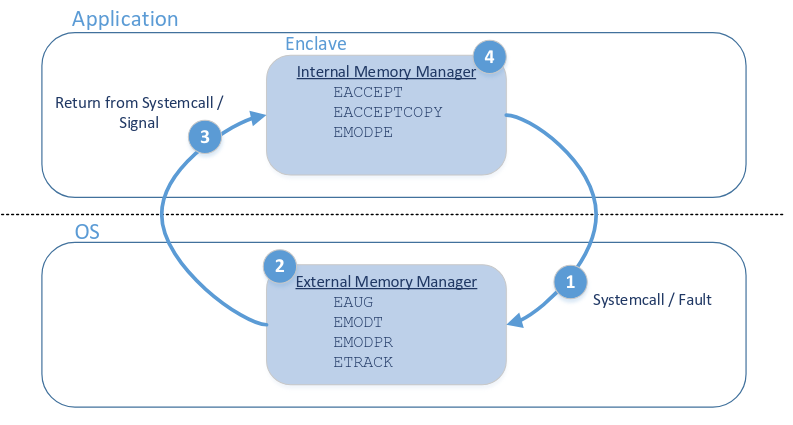
\includegraphics[width=.65\textwidth]{figures/ch1/sgx2.png}
  \end{center}
  \caption{Gestione dinamica della memoria in SGX2}\label{fig:sgx2}
\end{figure}

\clearpage
\section{Strumenti}
\subsection{Classificazione}\label{sec:classification}
Gli strumenti utilizzati per realizzare applicazioni \textit{trusted} che operano in TEE sono diversi e possono essere classificati secondo diversi criteri:
\begin{itemize}
  \item astrazione dall'architettura hardware: alcuni strumenti si interpongono al sistema operativo fornendo un insieme di ABI riscritte su cui si effettuano dei controlli o, come nel caso di \textit{occlum} fornisce un insieme di servizi che le applicazioni possono usare;
  \item trasparenza con il codice sorgente: alcuni strumenti come \textit{open enclave} richiede una ristrutturazione dell'applicazione in cui si distinguono chiaramente le parti sicure da quelle non sicure avendo come granularità la funzione;
\end{itemize}

Una panoramica degli strumenti analizzati è riportata in \cref{tab:TEE_tools_comparison}.

\begin{table}[h]
\centering
\begin{tabular}{|c|p{6cm}|p{6cm}|}
\hline
      & \textbf{Astrazione dall'architettura hardware} & \textbf{Trasparenza con il codice sorgente} \\ \hline
\textbf{Intel SGX SDK}  & Specifico per SGX, fornisce un insieme completo di API per sfruttare direttamente le capacità hardware di Intel SGX. & Richiede la divisione esplicita tra codice sicuro (enclave) e non sicuro, con un maggiore onere per lo sviluppatore. \\ \hline
\textbf{Rust SGX} & Specifico per SGX. Implementa un target diverso per il compilatore Rust & Supporta solo applicazioni scritte un Rust \\ \hline
\textbf{Open Enclave SDK} & Supporta diverse architetture hardware (ad es. Intel SGX, ARM TrustZone) attraverso un'astrazione comune. & Richiede una chiara distinzione tra le funzioni sicure e non sicure nel codice sorgente, con una ristrutturazione esplicita. \\ \hline
\textbf{Gramine-SGX}   & Implementa un livello di compatibilità (libOS) per eseguire applicazioni non modificate in SGX, rendendole indipendenti dall'hardware sottostante. & Non necessita di modifiche al codice sorgente dell'applicazione, facilitando l'integrazione di software legacy. \\ \hline
\textbf{Occlum}         & Fornisce un insieme di ABI riscritte e servizi di runtime per operare in TEE, semplificando l'implementazione e l'adattamento al TEE specifico. & L'applicazione non richiede modifiche significative al codice, poiché Occlum maschera le complessità dell'hardware sottostante. \\ \hline
\textbf{Enarx}          & Astratto rispetto all'hardware, utilizza WebAssembly come formato intermedio, garantendo portabilità su diversi TEE. & Le applicazioni devono essere portate in WebAssembly, richiedendo un adattamento potenzialmente significativo al codice. \\ \hline
\textbf{EGo} & Specifico per SGX. Esegue applicazioni GO in un enclave. & Richiede modifiche minimali al codice. Non supporta il multiprocessing e altre funzionalità di sistem.a \\ \hline
\textbf{MysticOS} & Sistema operativo leggero, basato su Open Enclave. Quindi si propone di essere \textit{hardware-agnostic} & Comporta molte limitazioni per la comunicazione con il sistema operativo. \\ \hline
\end{tabular}
\caption{Confronto tra strumenti per lo sviluppo di applicazioni trusted in TEE}
\label{tab:TEE_tools_comparison}
\end{table}

\subsection{Gramine}\label{sec:gramine}
Gramine\cite{GramineDocs} (ex Graphene) è un \textbf{libOS} che fornisce un'astrazione di alto livello in ambiente Linux per l'esecuzione di applicazioni isolate. Gramine è stato introdotto pre-SGX, ma è stato integrato con il concetto di enclave con \textbf{Gramine-SGX}. L'idea principale è quella di rendere applicazioni sicure senza modificare il codice sorgente, ma di effettuare un \textit{wrap} di un eseguibile in un ambiente isolato utilizzando SGX. 
L'astrazione principale di Gramine è il \textit{picoprocesso}\cite{Tsai2017}. Gramine inietta un componente detto \textbf{PAL} (\textit{Platform Abstraction Layer}) che si occupa di intercettare le \textit{system call} dell'applicazione e gestirle in modo sicuro garantendo che solo le operazioni autorizzate vengano eseguite. 

Di seguito, una panoramica di tutti gli elementi configurabili attraverso il \textbf{\textit{manifest file}}.
\begin{itemize}
  \item \textbf{\textit{loader}}: Carica l'applicazione nell'enclave, gestendo l'eseguibile principale le variabili d'ambiente;
  \item \textbf{\textit{libos}}: libOS emula un mini sistema operativo all'interno dell'enclave, permettendo all'applicazione intercettando le chiamate di sistema illegali all'interno dell'enclave ed implementa il protocollo previsto per comunicare tra mondo sicuro e non;
  \item \textbf{\textit{sgx}}: contiene le impostazioni specifiche per l'enclave SGX, inclusa la modalità di debug, la dimensione dell'enclave e i file trusted;   
  \item \textbf{\textit{fs}}: definisce come i file e le directory sono montati all'interno dell'enclave, permettendo di specificare percorsi di file system virtuali e di configurare mount point cifrati per proteggere i dati sensibili;
  \item \textbf{\textit{sys}}: gestisce le impostazioni di sistema per l'enclave, inclusa la dimensione dello stack e la configurazione di nomi di dominio runtime aggiuntivi;
\end{itemize}

\subsubsection{Struttura di un'applicazione con Gramine}
Come detto in \cref{sec:classification}, Gramine non prevede nessuna modifica al codice sorgente, ma prevede una specifica statica di tutti gli elementi dell'enclave attraverso un \textbf{\textit{manifest}}. Il manifest contiene informazioni per configurare il libOS e per configurare l'enclave fornendo opzioni come \textit{stack size} e \textit{enclave size}. Inoltre, contiene una lista di tutti i \textit{file} a cui può accedere l'enclave.

Il manifest è un \textit{file} in formato \textbf{\textit{toml}}. Attraverso l'utility \textit{gramine-manifest}, il manifest può essere personalizzato usando un template \textit{jinja} che supporta costrutti iterativi e condizionali e offre un meccanismo per iniettare variabili all'interno del file. In \cref{lst:basic-manifest}, è riportato un esempio minimale di manifest file. L'entrypoint è un eseguibile chiamato \textit{program} che deve essere necessariamente specificato come \textbf{\textit{trusted\_file}}. Se l'enclave accede ad un file non \textit{trusted} si verificherà un errore.

\begin{lstlisting}[caption=Esempio minimale di manifest file,label=lst:basic-manifest, language=Toml]
libos.entrypoint = "/program"

loader.env.LD_LIBRARY_PATH = "/lib"

fs.mounts = [
  { path = "/lib", uri = "file:{{ gramine.runtimedir() }}" },
  { path = "/program", uri = "file:program" },
]

sgx.trusted_files = [
  "file:program",
  "file:{{ gramine.runtimedir() }}/",
]
\end{lstlisting}
A partire dal file processato (viene calcolato un \textit{hash} (sha256) per tutti i file trusted), è possibile firmare il manifest con una chiave \textit{rsa} a $3072-bit$ ed eseguire l'enclave. 

Un manifest file più complicato è mostrato in \cref{lst:advanced-manifest}. I \textit{mount point} possono essere di diverso tipo. Ad esempio, \textit{tmpfs} è un file system in memoria privato all'enclave cifrato; \textit{encrypted} specifica che i file sono cifrati su disco e vengono acceduti da gramine in maniera trasparente. I mountpoint cifrati  possono specificare una chiave inserendola nel manifest (altamente insicuro) o indicare il nome di una chiave ottenuta con l'attestazione remota e devono essere dedicati per enclave. Quando non specificato, il mountpoint è di tipo \textit{chroot} che in maniera simile a come avviene in Linux permette di collegare file all'interno dell'ambiente dell'enclave. SGX consente la presenza di file non controllati condivisi con l'host con l'opzione \textit{sgx.allowed\_files}.

Infine, è possibile configurare opzioni per la dimensione dello stack e dell'enclave.

\begin{lstlisting}[caption="Manifest con allowed\_files\,mountpoint di diversa e configurazione per l'enclave",label=lst:advanced-manifest, language=Toml]
libos.entrypoint = "/program"

loader.env.LD_LIBRARY_PATH = "/lib"

sys.stack.size = "2M"
sys.enable_extra_runtime_domain_names_conf = true

sgx.debug = true
sgx.edmm_enable = {{ 'true' if env.get('EDMM', '0') == '1' else 'false' }}
sgx.enclave_size = "1G"

fs.mounts = [
  { path = "/lib", uri = "file:{{ gramine.runtimedir() }}" },
  { path = "/program", uri = "file:program" },
  { type = "tmpfs", path = "/tmp" },
  { type = "encrypted", path = "/encrypted/", uri = "file:encrypted/" },
]
fs.insecure__keys.default = "<hardcoded-key>"

sgx.trusted_files = [
  "file:program",
  "file:{{ gramine.runtimedir() }}/",
]

sgx.allowed_files = [
  "file:shared/"
]
\end{lstlisting}

\subsubsection{Remote attestation}
Come approfondito in \cref{sec:dcap-infrastructure-configuration}, la procedura con EPID è deprecata in favore della \textbf{\textit{Data Center Attestation Primitives} (DCAP)}. Gramine costruisce API di alto livello basate sulla remote attestation per creare facilmente tunnel TLS e fornire alle \textit{enclave} segreti. Gramine espone $3$ livelli di astrazione per fare utilizzare l'attestazione remota:
\begin{itemize}
  \item Low level interface: utilizza i pseudo files in Linux per eseguire le istruzioni SGX come EREPORT per generare quoting e report comunicando con le \textit{architectural enclave};
  \item RA-TLS: un insieme di due librerie utilizzate per aggiungere e verificare un SGX quote all'interno di un certificato X.509;
  \item Secret Provisioning: un API di alto livello per generare un segreto condiviso tra due applicazioni;
\end{itemize}
Per utilizzare l'attestazione, bisogna aggiungere \textbf{\textit{sgx.remote\_attestation}} nel manifest e impostare il tipo di attestazione utilizzata (al momento solo DCAP) come di seguito. 
\begin{verbatim}
sgx.remote_attestation = "dcap"
\end{verbatim}
\paragraph{Low-level interface}
L'enclave che utilizza la remote attestation può accedere ai file speciali in \textbf{\textit{/dev/attestation}} (riportati di seguito). 

\begin{forest}
  for tree={
    font=\ttfamily,
    grow'=0,
    child anchor=west,
    parent anchor=south,
    anchor=west,
    calign=first,
    edge path={
      \noexpand\path [draw, \forestoption{edge}]
      (!u.south west) +(7.5pt,0) |- node[fill,inner sep=1.25pt] {} (.child anchor)\forestoption{edge label};
    },
    before typesetting nodes={
      if n=1
        {insert before={[,phantom]}}
        {}
    },
    fit=band,
    before computing xy={l=15pt},
  }
  [dev/attestation/
  [attestation\_type]
  [user\_report\_data]
  [target\_info]
  [my\_target\_info]
  [report]
  [quote]
  [keys
    [default]
    [<key names>]
  ]
]
\end{forest}

Lo pseudo-file \textbf{\textit{report}} contiene il report SGX generato a partire dal contenuto in \textbf{\textit{user\_report\_data}} (contiene una stringa di questo inclusa nel report di $64B$) e \textbf{\textit{target\_info}} (contiene $512B$ di dati contenenti al target info). Il file \textbf{\textit{attestation\_type}} contiene il nome dello schema di attestazione in uso. Infine, l'SGX quote può essere letto da \textbf{\textit{/dev/attestation/quote}}. Quando si comunica con i dispositivi virtuali, SGX utilizza le istruzioni privilegiate come EREPORT e permette di comunicare con le \textit{architecturale enclave} (quali \textit{Quoting Enclave, Provisioning Certificate Enclave}) attraverso il \textbf{\textit{Architectural Enclave Service Manager} (AESM)}.

Infine, nella cartella \textit{keys} sono presenti le chiavi di crittografia ottenute da un servizio remoto come file binari di $128-bit$. 
\paragraph{RA-TLS}
Gramine utilizza le API di basso livello per fornire la possibilità di creare un tunnel TLS attestato con \textbf{\textit{RA-TLS}}: un insieme di due librerie che integra il protocollo TLS aggiungendo informazioni sul \textit{quote} all'interno del certificato \textbf{\textit{X.509}} (\cref{fig:ra-tls-certificate}). Le funzioni sono documentate in \textit{tools/sgx/ra\_tls.h} in \cite{gramine-repo}
\begin{itemize}
  \item \textbf{\textit{ra\_tls\_attest.so}}: contiene la funzione \textit{ra\_tls\_create\_key\_and\_crt\_der()} che serve ad aggiungere il quote in un certificato self-signed
  \item \textbf{\textit{ra\_tls\_verify\_dcap.so}}: contiene la funzione \textit{ra\_tls\_verify\_callback\_der()} utilizzata dal client per verificare il certificato. Anche se è possibile specificare una callback per verificare la callback, la funzione confronta i dati ricevuti dal server con le variabili d'ambiente \textbf{\textit{RA\_TLS\_*}} (MRENCLAVE, MRSIGNER, IS\_PROV\_ID);
\end{itemize}

\begin{figure}
  \begin{center}
    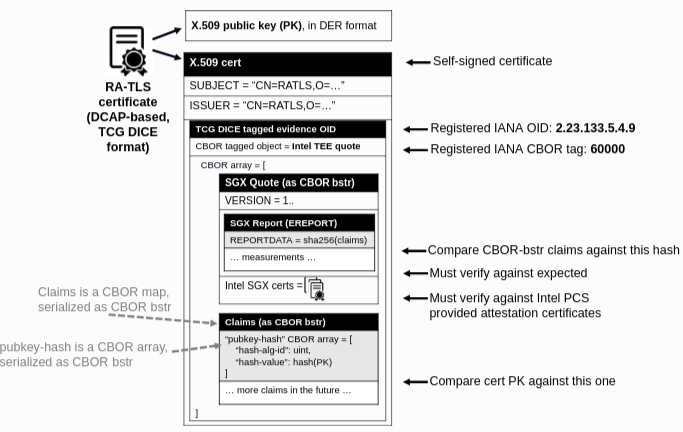
\includegraphics[width=0.95\textwidth]{figures/ch3/ra-tls-certificate.png}
  \end{center}
  \caption{Certificato X.509 arricchito con i dati del report SGX}\label{fig:ra-tls-certificate}
\end{figure}


\paragraph{Secret provisioning}
La secret provisioning è un'API di alto livello fornita attraverso due librerie e permette a due applicazioni che eseguono in TEE di negoziare segreti condivisi utilizzando la RA-TLS. Il caso d'uso più semplice è quello di un'applicazione client eseguita in un'enclave che riceve da un server delle chiavi per decifrare delle immagini o un modello. 

Le librerie fornite sono:
\begin{itemize}
  \item \textbf{\textit{secret\_prov\_attest.so}}: libreria utilizzata dal client. Una volta terminato il provisioning, il segreto viene fornito nella variabile d'ambiente \textit{SECRET\_PROVISIONING\_SECRET\_STRING}. Inoltre, la chiave viene salvata in \textit{/dev/attestation/keys/key-name};
  \item \textbf{\textit{secret\_prov\_verify\_dcap.so}}: libreria utilizzata dal server (che non esegue in un enclave) che richiama RA-TLS per verificare la firma del client.
\end{itemize}

\subsection{OpenEnclave}
Open enclave è un progetto che astrae il concetto di enclave proposto da Intel SGX in modo da renderlo \textit{hardware-agnostic} con l'intenzione di portarlo su altre piattaforme come ARM Trustzone. Come riportato in \cref{tab:tee-implementations}, Open Enclave richiede di suddividere il codice sorgente in \textit{enclave} (trusted) e \textit{host} (non trusted) con delle funzioni esplicite per l'esecuzione dell'enclave. In particolare, l'idea principale consiste nel generalizzare l'SDK proposta di Intel per SGX\cite{IntelSDK}.

\subsubsection{Struttura di un'applicazione con Open Enclave}
L'applicazione viene definita mediante un \textit{file} scritto in \textbf{\textit{Enclave Definition Language} (EDL)} definito da Intel nell'SDK\cite{IntelSDK}. Il linguaggio consente di importare altre definizioni e definisce una separazione netta tra parte sicura e parte non sicura. Come mostrato in \cref{lst:base-edl}, è riportato un esempio in cui si definiscono $2$ funzioni:
\begin{itemize}
  \item \textit{enclave\_helloworld()}: funzione da eseguire nell'enclave;
  \item \textit{host\_helloworld()}:  funzione host non sicura;
\end{itemize}
L'enclave importa delle definizioni standard come le \textit{syscall} in cui è implementato il meccanismo di comunicazione tra \textit{secure world} e \textit{non secure world}. Inoltre, può essere anche importata una libreria condivisa tra le due parti.

\begin{lstlisting}[caption=Esempio base di un file EDL,label=lst:base-edl]
enclave {
    from "openenclave/edl/syscall.edl" import *;
    from "platform.edl" import *;
     
    include "shared.h"

    trusted {
        public void enclave_helloworld();
    };

    untrusted {
        void host_helloworld();
    };
};
\end{lstlisting}

Analogamente a come avviene per IntelSDK, il file viene usato per generare tutte le funzioni e le definizioni su cui strutturare l'applicazione con l'utility \textit{oeedger8r}, come mostrato in \cref{sec:openenclave-helloworld}.

\subsubsection{Attestazione}
In OpenEnclave, l'attestazione remota è supportata solo per le macchine in Azure. Pertanto, gli esempi non includono la parte di comunicazione con i servizi remoti. Sebbene in modo più complicato, OpenEnclave crea un'astrazione simile a RA-TLS che può essere utilizzata per generare negoziare un segreto tra due enclave.

\clearpage
\section{Sviluppo di un'applicazione sicura}
In questa sezione, sono proposti $3$ esempi di applicazioni con SGX riportati in \cite{example-repo}:
\begin{itemize}
  \item \textbf{\textit{helloworld}}: applicazione di base che stampa a video un messaggio di benvenuto sia con Gramine che OpenEnclave;
  \item \textbf{\textit{attestation}}: esplorazione delle diverse API offerte da Gramine per l'attestazione includendo la condivisione di un segreto tra due applicazioni;
  \item \textbf{\textit{data sealing}}: applicazione che cifra i dati \textit{at rest} (sul disco) utilizzando le chiavi generate dall'enclave;
\end{itemize}

\subsection{Setup di laboratorio}
Gli esempi che seguono sono stati realizzati utilizzando il setup riportato in \cref{tab:lab-spec}.Come indicato in , esistono $2$ tipi di remote attestation: \textbf{\textit{Enhanced Privacy ID} (EPID)} e \textbf{\textit{Data Center Attestation Primitives} (DCAP)}. EPID incarica la QE di mettersi in contatto con l'\textbf{\textit{Intel Attestation Service} (IAS)} per avviare un algoritmo che consente di verificare la TCB. Purtroppo, questo meccanismo (più semplice da configurare) è stato deprecato e l'IAS sarà chiuso definitivamente in data \textit{2 aprile 2025}. L'unica modalità di fare attestazione remota è quella di configurare DCAP con uno sforzo infrastrutturale del cloud provider. Questa scelta è data anche dalla volontà di Intel di unificare i servizi di remote attestation tra SGX e TDX.

\begin{table}[h]
\centering
\begin{tabular}{|l|p{7cm}|}
\hline
 Componente & Descrizione \\ \hline
\textbf{CPU} & i7-9700 CPU @ 3.00GHz, SGX1 e FLC  \\ \hline
\textbf{RAM} & 24 GB, 2666 MT/s DDR4 \\ \hline
\textbf{OS} & Ubuntu 24.04 LTS, kernel 6.8.0-41-generic \\ \hline
\textbf{Platform} & Dell Opitplex-7070 \\ \hline
\textbf{SGX SDK version} & 2.25 \\ \hline
\textbf{SGX DCAP version} & 1.22 \\ \hline
\textbf{Docker version} & 27.3.1 \\ \hline
\textbf{Gramine Version} & v1.8 \\ \hline
\textbf{OpenEnclave Version} & v0.19.8 \\ \hline
\end{tabular}
\caption{Caratteristiche tecniche macchina di laboratorio}
\label{tab:lab-spec}
\end{table}

Sia Gramine che OpenEnclave necessitano di componenti specifiche per la versione di Ubuntu utilizzata. Per assicurare la riproducibilità degli esperimenti, è stato utilizzato Docker. A partire dal kernel 5.11, SGX con l'attestazione DCAP è incluso come driver in upstream e, pertanto, non necessita di installazioni. In particolare, sono forniti due dispositivi Linux che devono essere utilizzati all'interno dei container per accedere alle istruzioni SGX: \textbf{\textit{/dev/sgx\_enclave}} e \textbf{\textit{/dev/sgx\_provision}}. Il codice sorgente dei driver e dell'SDK è riportato in \cite{linux-sgx}.

\subsubsection{Installazione Gramine}
Per usare correttamente le primitive DCAP, è necessario compilare da codice sorgente Gramine con il flag \textit{-Ddcap=enabled}. Per rendere riproducibile la procedura di compilazione, installazione e configurazione è stato sviluppato un Dockerfile (riportato in \cref{lst:gramine-sdk-dockerfile}). È possibile creare un'immagine con:
\begin{verbatim}
 docker build -t gramine-dcap . 
\end{verbatim}
\lstinputlisting[caption=Dockerfile per la creazione di un ambiente di sviluppo riproducibile con Gramine,label=lst:gramine-sdk-dockerfile,language=docker]{../gramine/Dockerfile}

\begin{verbatim}
 docker run \
  -it \
  --network=host \
  --device /dev/sgx_enclave \ 
  --device /dev/sgx_provision \
  gramin-dcap
\end{verbatim}

\subsubsection{Installazione Open Enclave} OpenEnclave è supportato solo con Ubuntu 20.04 a causa di alcune dipendenze con OpenSSL. Per questo motivo, l'SDK è stata installata utilizzando un container \textit{Docker} utilizzando il Dockerfile (creato a partire dalla documentazione \cite{openenclave}) in \cref{lst:openenclave-sdk-dockerfile}. A partire da questo Dockerfile, può essere creata un'immagine con (supponenedo di essere nella stessa cartella del file):
\begin{verbatim}
 docker build -t openenclave-sdk .
\end{verbatim}

\lstinputlisting[caption=Dockerfile per la creazione di un ambiente di sviluppo riproducibile con OpenEnclave SDK,  label=lst:openenclave-sdk-dockerfile,language=docker]{../openenclave/Dockerfile}

Creata l'immagine, è possibile avere un terminale interattivo all'interno di un container condividendo il codice sorgente dell'applicazione (supponendo di essere nella \textit{top-level directory}) del proprio progetto. 
\begin{verbatim}
 docker run \
  -it \
  --network=host \
  --device /dev/sgx_enclave \ 
  --device /dev/sgx_provision \
  openenclave-sdk \ 
\end{verbatim}

\subsubsection{Configurazione infrastruttura DCAP}\label{sec:dcap-infrastructure-configuration}
L'infrastruttura DCAP (\cref{fig:dcap-infra}) mira a minimizzare le interazioni con i servizi remoti di Intel concentrando la gestione dei certificati su un componente \textit{trusted} detto \textbf{\textit{Provisioning Certificate Caching Service} (PCCS)}. Il PCCS è l'unico componente dell'infrastruttura che può interagire con i servizi di Intel (attraverso una API Key, \cref{fig:intel-portal-registration}) e può essere contattato direttamente dai quoting enclave delle singole macchine come un servizio HTTP. A partire dalla versione DCAP 1.22, Intel non offre più un'implementazione di riferimento di questo servizio, ma rimane comunque accessbile dalle release precedenti. Tutte le informazioni riportate sono state ottenute dai documenti e dal codice sorgente rilasciati da Intel\cite{sgx-dcap-docs},\cite{sgx-dcap-repo}.

\begin{figure}[H]
  \begin{center}
    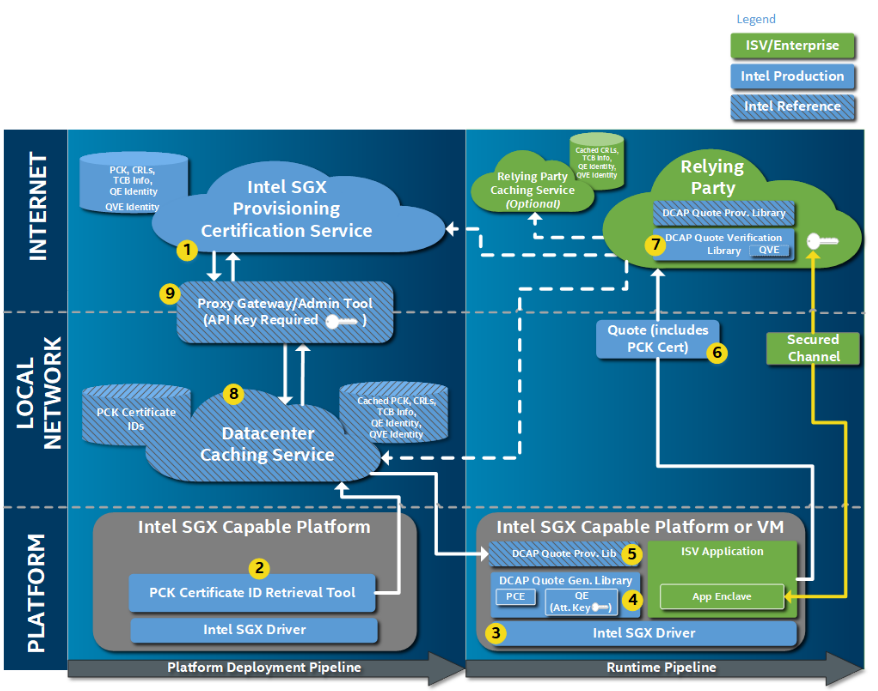
\includegraphics[width=.7\textwidth]{figures/ch3/dcap-infra.png}
  \end{center}
  \caption{Diagramma di infrastruttura DCAP}\label{fig:dcap-infra}
\end{figure}

Le API Key possono essere ottenute registrando un account su questo \href{https://api.portal.trustedservices.intel.com}{portale}.

\begin{figure}[h]
\centering
\begin{subfigure}{.5\textwidth}
  \centering
  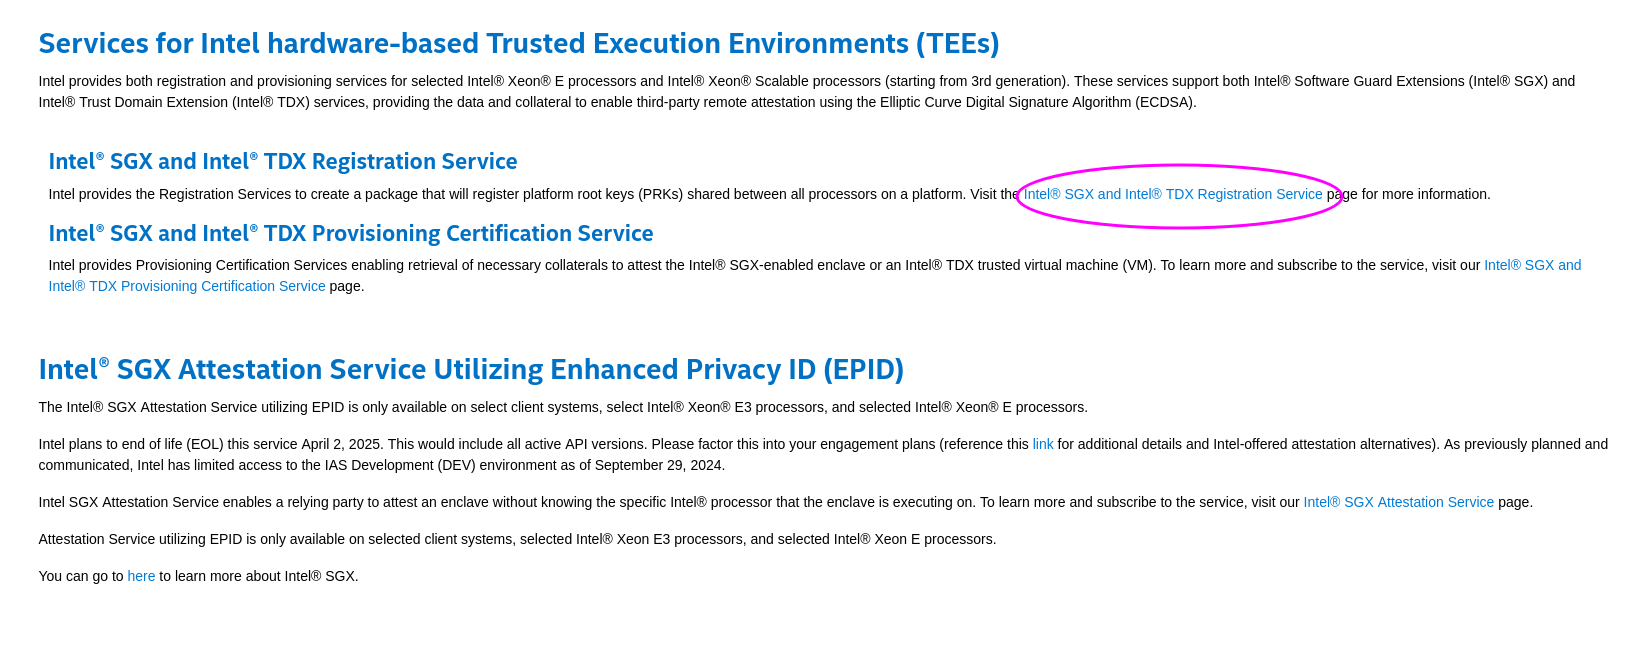
\includegraphics[width=.95\textwidth]{figures/ch3/intel-portal-1.png}
  \caption{Navigazione sul sito}
\end{subfigure}%
\begin{subfigure}{.5\textwidth}
  \centering
  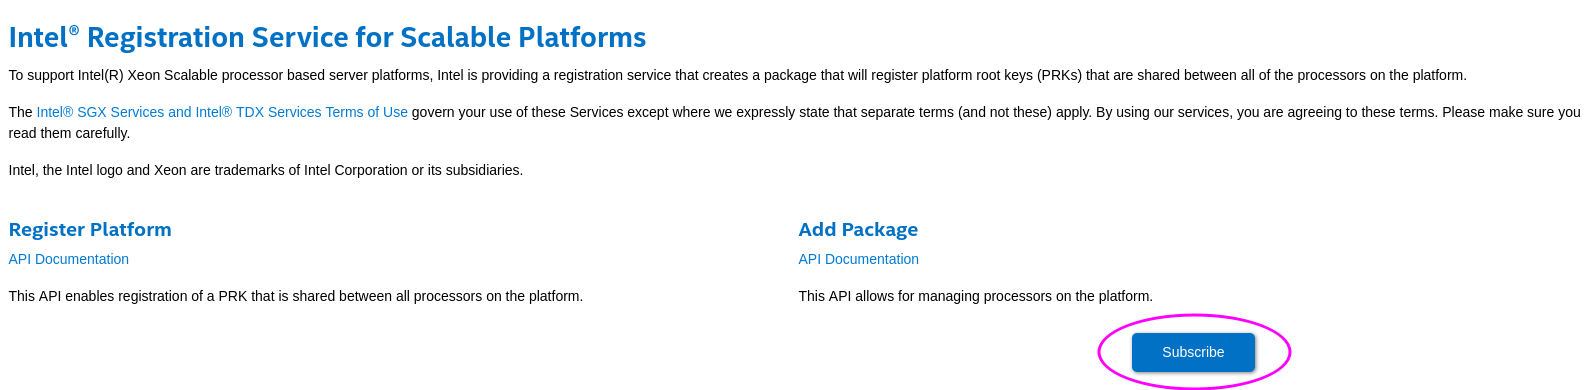
\includegraphics[width=.95\textwidth]{figures/ch3/intel-portal-2.png}
  \caption{Click sul pulsante subscribe}
\end{subfigure}
\begin{subfigure}{.5\textwidth}
  \centering
  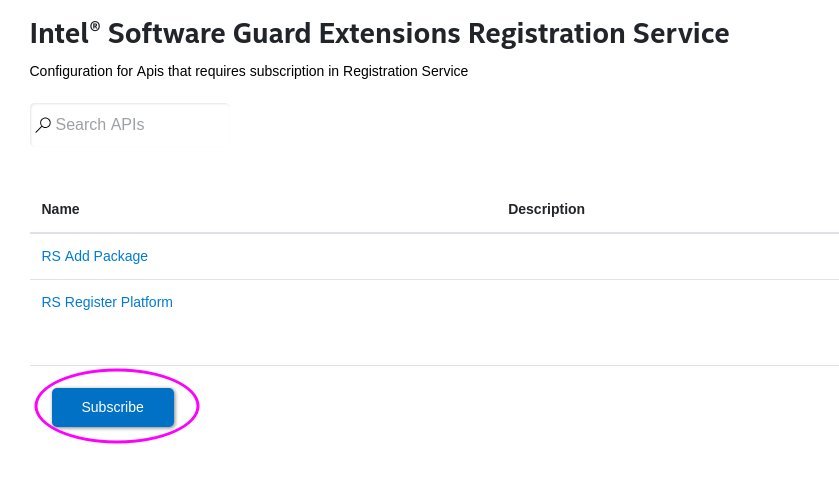
\includegraphics[width=.95\textwidth]{figures/ch3/intel-portal-3.png}
  \caption{Creazione API Key}
\end{subfigure}
\caption{Procedura di registrazione sul sito Intel}
\label{fig:intel-portal-registration}
\end{figure}

\paragraph{Configurazione host}
Anche se si utilizzano ambienti containerizzati, bisogna configurare l'host con i permessi per accedere ai device Linux che si occupano di generare report. In particolare, come mostrato di seuito, bisogna configurare i permessi sui driver di \textbf{\textit{sgx\_enclave}} \textbf{\textit{sgx\_provision}} (implementati già nel kernel Linux) conferendo l'accesso in lettura e scrittura per gli utenti appartenenti al gruppo \textbf{\textit{sgx\_prv}}. Per fare questo, aggiungere nel file \textbf{/etc/udev/rules.d/90-sgx-v40.rules} le seguenti espressioni:
\begin{verbatim}
SUBSYSTEM=="misc",KERNEL=="sgx_enclave",MODE="0666",SYMLINK+="sgx/enclave"
SUBSYSTEM=="misc",KERNEL=="sgx_provision",GROUP="sgx_prv",MODE="0660",SYMLINK+="sgx/provision"
\end{verbatim}
e ricaricare le regole con:
\begin{verbatim}
udevadm trigger
\end{verbatim}

Dopo queste modifiche, bisogna aggiungere qualsiasi utente (incluso root in un container Docker) al gruppo \textit{sgx\_prv}. Se si utilizzano i Dockerfile mostrati in precedenza, l'utente root è già stato configurato correttamente. 
  
\paragraph{Installazione PCCS}
Intel specifica l'architettura del PCCS in e fino alla versione 1.21 DCAP fornisce\\ un'implementazione di riferimento. Di seguito, si riporta la procedura di installazione e configurazione per quella implementazione.
Il PCCS è un'applicazione web scritta in Javascript e può essere trovata nel path \textbf{\textit{QuoteGeneration/pccs}} della repository nella versione 1.21. Prima di installare, bisogna ottenere delle API Key dal servizio Intel creando un account seguendo questa guida \cite{quickstart-dcap}. Per rendere riproducibile la compilazione di questo componente, è stato creato il Dockerfile in \cref{lst:pccs-dockerfile} con cui creare un'immagine:
\begin{verbatim}
docker build -t pccs . 
\end{verbatim}

\lstinputlisting[caption=Dockerfile per la compilazione del PCCS,  label=lst:pccs-dockerfile,language=docker]{../pccs/Dockerfile}

Il PCCS non è pensato per essere eseguito in un enclave, ma è una normale applicazione che espone delle API attraverso un tunnel TLS. Per eseguire un container con PCCS, bisogna creare una coppia di chiavi pubblica e privata da cui si genera un certificato:
\begin{verbatim}
openssl genrsa -out private.pem 2048
openssl req -new -key private.pem -out csr.pem
openssl x509 -req -days 365 -in csr.pem -signkey private.pem -out file.crt
\end{verbatim}

Inoltre, bisogna creare un file di configurazione in formato json simile a quello mostrato in \cref{lst:pccs-config}. Nell'esempio, viene utilizzato un database SQLite.

\lstinputlisting[caption=Esempio file di configurazione per PCCS,label=lst:pccs-config,language=toml]{../pccs/config/example.json}

Bisogna inserire in \textit{ApiKey} una delle due chiavi ricavate dalla piattaforma intel. Per \textbf{\textit{UserTokenHash}} e \textbf{\textit{AdminTokenHash}}, bisogna salvare l'hash con \textit{sha512} sostituendo le effettive password per nel seguente snippet:
\begin{verbatim}
echo -n "user_password" | sha512sum | tr -d '[:space:]-'
echo -n "admin_password" | sha512sum | tr -d '[:space:]-'
\end{verbatim}

Infine, è possibile eseguire l'applicazione (per semplificare le attività di deploy tutti i container eseguiti usano la rete dell'host):
\begin{verbatim}
docker run \ 
  -d \
  --network=host \
  -v $(pwd)/<path-to-config-file>:/app/config/default.json \
  -v $(pwd)/<path-to-certs-dir>:/app/ssl_key/ \ 
  pccs
\end{verbatim}

\paragraph{Configurazione AESM service}
Per usare correttamente, la remote attestation bisogna configurare ed utilizzare le \textbf{\textit{Architectural Enclave} (AE)} (come la \textbf{\textit{Quoting Enclave} (QE)}, \textbf{\textit{Quoting Verification Enclave} (QVE)}). Le \textit{architectural enclave} sono enclave privilegiate fornite e firmate da Intel che devono essere gestite da attraverso l'\textbf{\textit{Architectural Enclave Service Manager} (AESM)}. AESM è un'applicazione che espone i servizi delle architectural enclave attraverso una \textbf{\textit{unix socket}}. Queste enclave possono comunicare con il PCCS e vengono configurate attraverso il file \textbf{\textit{ /etc/sgx\_default\_qcnl.conf}} (riportato di seguito). Se si vuole comunicare con un PCCS che usa certificati \textit{self-signed}, bisogna impostare il flag \textbf{\textit{use\_secure\_cert}} a \textit{false}. AESM è installato sia nelle immagini di openenclave che gramine.

\begin{lstlisting}[caption=Configurazione remote attestation per le Architectural Enclaves,label=default-qcnl.conf,language=toml]
{
  // *** ATTENTION : This file is in JSON format so the keys are case sensitive. Don't change them.

  //PCCS server address
  "pccs_url": "https://localhost:8081/sgx/certification/v4/"

  // To accept insecure HTTPS certificate, set this option to false
  ,"use_secure_cert": true

  // You can use the Intel PCS or another PCCS to get quote verification collateral.  Retrieval of PCK
  // Certificates will always use the PCCS described in pccs_url.  When collateral_service is not defined, both
  // PCK Certs and verification collateral will be retrieved using pccs_url
  //,"collateral_service": "https://api.trustedservices.intel.com/sgx/certification/v4/"

  // Type of update to TCB Info. Possible value: early, standard. Default is standard.
  // early indicates an early access to updated TCB Info provided as part of a TCB recovery event
  // (commonly the day of public disclosure of the items in scope)
  // standard indicates standard access to updated TCB Info provided as part of a TCB recovery event
  // (commonly approximately 6 weeks after public disclosure of the items in scope)
  //, "tcb_update_type" : "standard"

  // If you use a PCCS service to get the quote verification collateral, you can specify which PCCS API version is to be used.
  // The legacy 3.0 API will return CRLs in HEX encoded DER format and the sgx_ql_qve_collateral_t.version will be set to 3.0, while
  // the new 3.1 API will return raw DER format and the sgx_ql_qve_collateral_t.version will be set to 3.1. The pccs_api_version
  // setting is ignored if collateral_service is set to the Intel PCS. In this case, the pccs_api_version is forced to be 3.1
  // internally.  Currently, only values of 3.0 and 3.1 are valid.  Note, if you set this to 3.1, the PCCS use to retrieve
  // verification collateral must support the new 3.1 APIs.
  //,"pccs_api_version": "3.1"

  // Maximum retry times for QCNL. If RETRY is not defined or set to 0, no retry will be performed.
  // It will first wait one second and then for all forthcoming retries it will double the waiting time.
  // By using retry_delay you disable this exponential backoff algorithm
  ,"retry_times": 6

  // Sleep this amount of seconds before each retry when a transfer has failed with a transient error
  ,"retry_delay": 10

  // If local_pck_url is defined, the QCNL will try to retrieve PCK cert chain from local_pck_url first,
  // and failover to pccs_url as in legacy mode.
  //,"local_pck_url": "http://localhost:8081/sgx/certification/v4/"

  // If local_pck_url is not defined, set pck_cache_expire_hours to a none-zero value will enable local cache.
  // The PCK certificates will be cached in memory and then to the disk drive.
  // The local cache files will be sequentially searched in the following directories until located in one of them:
  // Linux : $AZDCAP_CACHE, $XDG_CACHE_HOME, $HOME, $TMPDIR, /tmp/
  // Windows : $AZDCAP_CACHE, $LOCALAPPDATA\..\..\LocalLow
  // Please be aware that the environment variable pertains to the account executing the process that loads QPL,
  // not the account used to log in. For instance, if QPL is loaded by QGS, then those environment variables relate to
  // the "qgsd" account, which is the account that runs the QGS daemon.
  // You can remove the local cache files either manually or by using the QPL API, sgx_qpl_clear_cache. If you opt to
  // delete them manually, navigate to the aforementioned caching directories, find the folder named .dcap-qcnl, and delete it.
  // Restart the service after all cache folders were deleted. The same method applies to "verify_collateral_cache_expire_hours"
  ,"pck_cache_expire_hours": 168

  // To set cache expire time for quote verification collateral in hours
  // See the above comment for pck_cache_expire_hours for more information on the local cache.
  ,"verify_collateral_cache_expire_hours": 168

  // When the "local_cache_only" parameter is set to true, the QPL/QCNL will exclusively use PCK certificates
  // from local cache files and will not request any PCK certificates from service providers, whether local or remote.
  // To ensure that the PCK cache is available for use, an administrator must pre-populate the cache folders with
  // the appropriate cache files. To generate these cache files for specific platforms, the administrator can use
  // the PCCS admin tool. Once the cache files are generated, the administrator must distribute them to each platform
  // that requires provisioning.
  ,"local_cache_only": false

  // You can add custom request headers and parameters to the get certificate API.
  // But the default PCCS implementation just ignores them.
  //,"custom_request_options" : {
  //  "get_cert" : {
  //    "headers": {
  //      "head1": "value1"
  //    },
  //    "params": {
  //      "param1": "value1",
  //      "param2": "value2"
  //    }
  //  }
  //}
}
\end{lstlisting}

\clearpage
\subsection{Applicazione Helloworld}
In questo esempio, viene illustrato un programma minimale sia con Gramine che con Open Enclave con lo scopo di evidenziarne le differenze. Lo scopo del programma è quello di stampare a video un messaggio di benvenuto.
\subsubsection{Gramine}
Come detto in \cref{sec:gramine}, il codice sorgente dell'applicazione rimane invariato, ma bisogna focalizzarsi in sul manifest file, riportato di seguito.

\lstinputlisting[caption=Manifest per un semplice programma helloworld,label=lst:helloworld-manifest, language=Toml]{../gramine/examples/helloworld/helloworld.manifest.template}

La struttura della directory è riportata di seguito. La \textbf{\textit{toolchain}} Gramine riconosce l'applicazione dal nome del file manifest dato in ingresso. 

\begin{forest}
  for tree={
    font=\ttfamily,
    grow'=0,
    child anchor=west,
    parent anchor=south,
    anchor=west,
    calign=first,
    edge path={
      \noexpand\path [draw, \forestoption{edge}]
      (!u.south west) +(7.5pt,0) |- node[fill,inner sep=1.25pt] {} (.child anchor)\forestoption{edge label};
    },
    before typesetting nodes={
      if n=1
        {insert before={[,phantom]}}
        {}
    },
    fit=band,
    before computing xy={l=15pt},
  }
  [app/
    [helloworld.c]
    [Makefile]
    [helloworld.manifest]
  ]
]
\end{forest}

Il file in \cref{lst:helloworld-manifest} deve essere preprocessato e firmato con \textit{sgx}. Questa procedura crea un file chiamato \textit{helloworld.manifest} e la sua firma in \textit{helloworld.sign}. In \cref{lst:helloworld-makefile}, è riportato il \textit{Makefile} utilizzato per la compilazione dell'applicazione ed è possibile osservare che la generazione dell'eseguibile non dipende dalla parte. La regola per generare \textit{helloworld.manifest} utilizza \textit{gramine-manifest} che effettua un \textit{preprocessing} di \textit{helloworld.manifest.template}. Questo comando può definire variabili all'interno del manifest che poi saranno utilizzate con la sintassi di \textit{jinja}. Ad esempio, \textit{-Dlog\_level} definisce la variabile \textit{\{log\_level\}}.

\lstinputlisting[language=make, caption=Makefile per applicazione helloworld,label=lst:helloworld-makefile]{../gramine/examples/helloworld/Makefile}

Con \textit{gramine-sgx-sign} viene calcolata una firma dell'enclave cifrata con una chiave ottenuta eseguendo il comando \textit{gramine-sgx-gen-private-key} (che genera una chiave rsa a 3072 bit). In questa fase, il codice dell'enclave viene misurato insieme ad altri metadati per generare la \textit{SIGSTRUCT}. La genuinità di questa firma può essere verificata attraverso la \textit{remote attestation}. Successivamente, l'applicazione può essere eseguita con privilegi di amministratore usando il comando:
\begin{verbatim}
  $ gramine-sgx helloworld
\end{verbatim}
Dove \textit{helloworld} è il nome del manifest file privato delle estensioni. Analizzando il log della compilazione, Gramine mostra tutte le misure che effettua per ogni pagina di memoria. All'esecuzione, l'enclave viene creata (\cref{fig:gramine-helloworld-create-enclave}, i campi \textit{attr} sono relativi alla struttura \textit{SECS}, mentre con \textit{size} viene specificata quella riportata nel \textit{manifest}) e la sua memoria popolata pagina per pagina configurando i permessi di lettura/scrittura/esecuzione (RWX)(\cref{fig:gramine-helloworld-create-enclave-page-mapping}).

\begin{figure}
  \begin{center}
    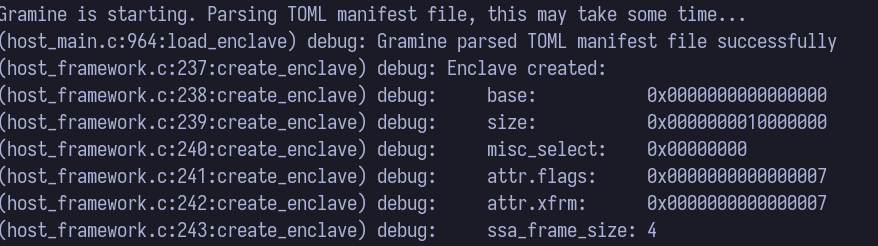
\includegraphics[width=.95\textwidth]{figures/ch3/gramine-helloworld-create-enclave.png}
  \end{center}
  \caption{Creazione dell'enclave con Gramine}\label{fig:gramine-helloworld-create-enclave}
\end{figure}

\begin{figure}[H]
  \begin{center}
    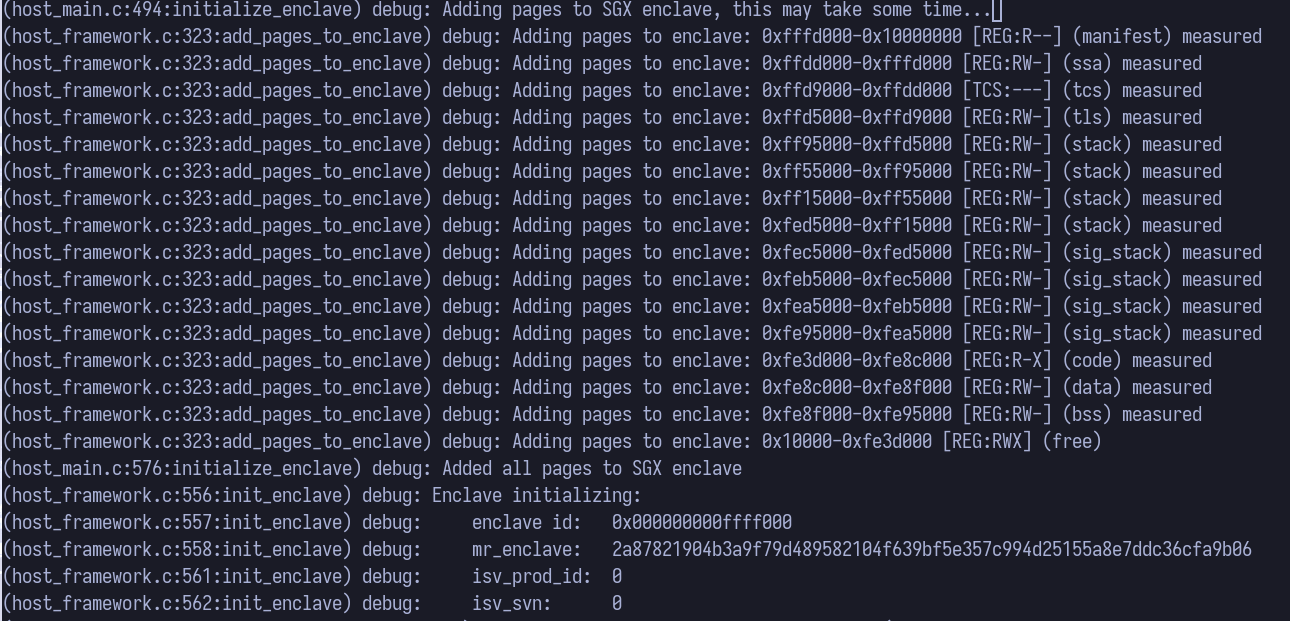
\includegraphics[width=0.95\textwidth]{figures/ch3/gramine-helloworld-create-enclave-page-mapping.png}
  \end{center}
  \caption{Mapping delle pagine}\label{fig:gramine-helloworld-create-enclave-page-mapping}
\end{figure}

Dopo aver caricato le pagine, viene inizializzato il \textit{libOs} che monta i file system ed esegue l'entrypoint.

\subsubsection{OpenEnclave}\label{sec:openenclave-helloworld}
L'applicazione base con Open Enclave risulta più complicata. Innanzitutto, bisogna specificare un file EDL come quello in \cref{lst:openenclave-helloworld-edl}. In particolare, questo definisce due funzioni (\textit{host\_helloworld e \textit{enclave\_helloworld}}) che l'enclave può eseguire in due differenti modalità e che devono essere implementate nell'applicazione finale.

\lstinputlisting[caption=EDL per applicazione helloworld,  label=lst:openenclave-helloworld-edl]{../openenclave/examples/helloworld/helloworld.edl}

Con OpenEnclave, c'è una separazione netta tra parte trusted e untrusted rispecchiata dalla struttura del progetto.

\begin{forest}
  for tree={
    font=\ttfamily,
    grow'=0,
    child anchor=west,
    parent anchor=south,
    anchor=west,
    calign=first,
    edge path={
      \noexpand\path [draw, \forestoption{edge}]
      (!u.south west) +(7.5pt,0) |- node[fill,inner sep=1.25pt] {} (.child anchor)\forestoption{edge label};
    },
    before typesetting nodes={
      if n=1
        {insert before={[,phantom]}}
        {}
    },
    fit=band,
    before computing xy={l=15pt},
  }
  [app/
  [host
  [host.c]
  [Makefile]
  ]
  [enclave
  [enc.c]
  [Makefile]
  ]
    [Makefile]
    [helloworld.edl]
  ]
]
\end{forest}

Prima di sviluppare l'applicazione, è necessario creare le definizioni di tipi e importare le funzioni principali di OpenEnclave. Principalmente, queste definizioni servono a facilitare la gestione del ciclo di vita dell'enclave (\cref{fig:enclave-lifecycle}), gestendo le ECALL e OCALL con opportune EENTER e EEXIT. Questo può essere fatto con \textit{oeedger8r} che prende in ingresso il file \textit{edl} e si occupa di definire i tipi giusti in base al \textit{backend} specificato. Ad esempio, per generare il codice relativo all'enclave bisogna eseguire (stando nella cartella \textit{enclave}):
\begin{verbatim}
  oeedger8r --search-path /opt/openenclave/include 
    --search-path /opt/openenclave/include/openenclave/edl/sgx
    ../helloworld.edl --trusted
\end{verbatim}

Per generare la parte untrusted, bisogna eseguire (stando nella cartella \textit{untrusted}):
\begin{verbatim}
  oeedger8r --search-path /opt/openenclave/include 
    --search-path /opt/openenclave/include/openenclave/edl/sgx
    ../helloworld.edl --untrusted
\end{verbatim}

Il Makefile principale si limita a richiamare gli altri file nelle rispettive sezioni dell'applicazione. 

\lstinputlisting[language=make,caption=Makefile helloworld con openenclave,captionpos=bottom]{../openenclave/examples/helloworld/Makefile}

\paragraph{Applicazione host} L'applicazione host gestisce il ciclo di vita dell'enclave dalla sua creazione alla distruzione. Il codice (in cui sono stati omessi i controlli degli errori per brevità) è riportato in \cref{lst:openenclave-helloworld-host}. Questo non cambia molto rispetto ad un'applicazione classica in $C$. La funzione \textit{oe\_create\_helloworld\_enclave} crea l'enclave e prende come primo parametro il path per l'enclave firmata definito nella macro \textit{ENCLAVE\_SIGNED\_PATH}. Alla creazione dell'enclave viene verificata la firma e viene popolata la EPC. La funzione \textit{enclave\_helloworld} è una funzione nella parte trusted che esegue nel TEE (una ECALL) alla quale corrisponde un cambio di contesto del processore. Infine, con \textit{oe\_terminate\_enclave}, si elimina l'enclave.

\lstinputlisting[language=C,caption=Codice principale applicazione host,label=lst:openenclave-helloworld-host]{../openenclave/examples/helloworld/host/host.c}

Questo componente è dotato di un Makefile, riportato in \cref{lst:openenclave-helloworld-host-makefile}, in cui si compila normalmente l'applicazione dopo aver generato i flag del compilatore a partire da \textit{open-enclave}. Il compilatore utilizzato è \textit{clang}, ma sono supportati anche \textbf{\textit{cc}} e \textbf{\textit{gcc}}. Per cambiare compilatore, bisogna modificare il valore della variabile \textit{CC} per ogni Makefile.

\lstinputlisting[language=make,caption=Makefile per la parte host,label=lst:openenclave-helloworld-host-makefile]{../openenclave/examples/helloworld/Makefile}

\paragraph{Applicazione enclave}
Per compilare l'enclave, bisogna seguire i seguenti passi racchiusi nel Makefile in \cref{lst:openenclave-helloworld-enclave-makefile}.
\begin{itemize}
  \item \textbf{\textit{compilare l'applicazione}}: procedimento standard che avviene specificato nella regola \textit{build}. Avviene analogamente alla parte host;
  \item \textbf{\textit{generare una coppia di chiavi}}: con la regola \textit{keys} si genera una chiave privata a $3072-$bit da cui se ne deriva una pubblica;
  \item \textbf{\textit{firmare l'applicazione}}: con \textit{oesign} nella regola \textbf{sign}, l'applicazione viene firmata con la chiave privata generata in precedenza e un file di configurazione riportato in \cref{lst:openenclave-helloworld-enclave-conf};
\end{itemize}

Il file di configurazione definisce alcuni parametri di configurazione per l'enclave ed è un semplice file di testo:
\begin{itemize}
  \item \textbf{\textit{debug}}: saranno stampate informazioni aggiuntive;
  \item \textbf{\textit{NumHeapPages}}: massimo numero di pagine nell'heap per ogni thread nell'enclave;
  \item \textbf{\textit{NumStackPages}}: massimo numero di pagine nello stack per ogni thread nell'enclave;
  \item \textbf{\textit{NumTCS}}: massimo numero di \textbf{\textit{Thread Control Structure}} consentito nell'enclave;
  \item \textbf{\textit{ProductID}}: definisce un identificativo univoco per l'applicazione in modo tale da poter distinguire due programmi firmati dallo stesso \textit{MRSIGNER};
  \item \textbf{\textit{SecurityVersion}}: protegge contro gli attacchi di tipo \textbf{\textit{rollback}};
\end{itemize}

\lstinputlisting[language=Ini,caption=Configurazione per la generazione dell'enclave,label=lst:openenclave-helloworld-enclave-conf]{../openenclave/examples/helloworld/enclave/helloworld.conf}

L'applicazione utilizza una versione minimale tls chiamata \textbf{\textit{mbed-tls}}, ma potrebbe essere usata \textbf{openssl} assegnando alla variabile \textit{CFLAGS} il valore ottenuto dal comando:

\begin{verbatim}
pkg-config oeenclave-clang --variable=openssl_3flags 
\end{verbatim}

\lstinputlisting[language=make,caption=Makefile per la parte enclave,label=lst:openenclave-helloworld-enclave-makefile]{../openenclave/examples/helloworld/enclave/Makefile}

Il codice \textit{enc.c}, riportato \cref{lst:openenclave-helloworld-enclave}, non contiene un \textit{main}, ma solo la funzione da eseguire nel TEE. La funzione \textit{host\_helloworld} è una OCALL e comporta un'uscita dall'enclave per entrare nella parte untrusted ed è definita nel parte \textit{host}.

\lstinputlisting[language=C,caption=Codice principale applicazione enclave,label=lst:openenclave-helloworld-enclave]{../openenclave/examples/helloworld/enclave/enc.c}

\subsection{Applicazione Attestation}
Gli esempi che interagiscono con la parte di attestazione remota. Con Gramine, vengono esplorate le API di \textit{secret provisioning} oltre a quelle di generazione di \textit{report} e \textit{quote}.

\subsubsection{Gramine}
\paragraph{Low-level interface}
In \cref{lst:low-level-attestation}, è riportato un'applicazione demo in Python che interagisce con i file descritti in precedenza generando e stampando a video report e quote (la decodifica è stata fatta in base ai documenti in \cite{IntelSDK}). 

\lstinputlisting[language=python, caption=Interazione con i file per l'attestazione remota,label=lst:low-level-attestation]{../gramine/examples/remote-attestation/main.py}

Inoltre, bisogna modificare il manifest file aggiungendo tutti i file necessari ad eseguire un'istanza dell'interprete python e specificare il tipo di attestazione richiesta.

\lstinputlisting[language=python, caption=Manifest file per l'esecuzione di un interprete Python=lst:low-level-attestation-manifest-file]{../gramine/examples/remote-attestation/ra.manifest.template}

Il Makefile è analogo al caso precedente. Il risultato è riportato in \cref{fig:ra-low-level-example}.

\begin{figure}[H]
  \begin{center}
    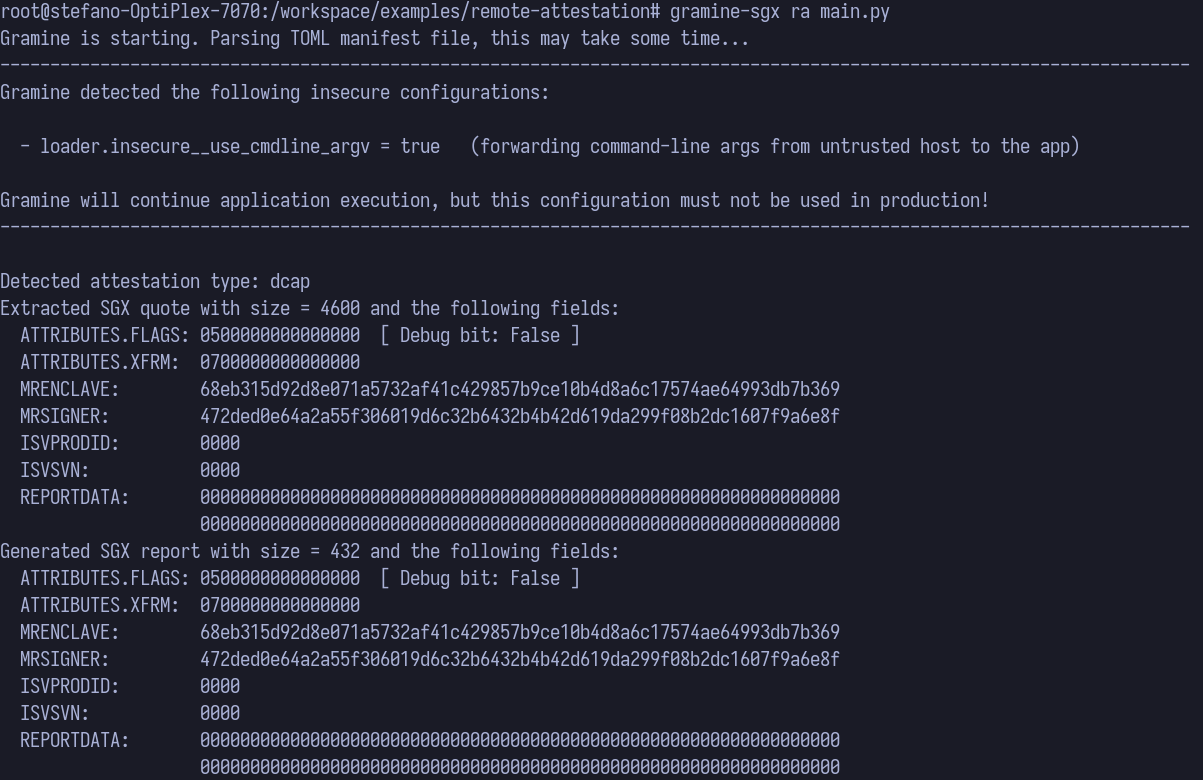
\includegraphics[width=0.95\textwidth]{figures/ch3/ra-low-level-example.png}
  \end{center}
  \caption{Lettura del Quote e del Report attraverso i file virtuali in Linux}\label{fig:ra-low-level-example}
\end{figure}

\paragraph{RA-TLS}
Gramine non effettua nessuna scelta sull'implmentazione TLS da utilizzare (è possibile utilizzare sia OpenSSL che mbedtls). Il codice mostrato è tratto dall'esempio "ra-tls-mbedtls". Il server deve essere eseguito in un enclave; mentre il client può essere un'applicazione normale (può essere eseguito in un enclave). Una volta compilata l'applicazione con

\begin{verbatim}
make clean app dcap 
\end{verbatim}

bisogna ottenere le informazioni da passare al client per verificare la firma del server. Questo può essere fatto con il tool \textit{gramine-sgx-sigstruct-view}. 

Per esempio può essere eseguita una demo con 
\begin{verbatim}
gramine-sgx ./server &

RA_TLS_MRENCLAVE=<MRENCLAVE of the server enclave> \
RA_TLS_MRSIGNER=<MRSIGNER of the server enclave> \
RA_TLS_ISV_PROD_ID=<ISV_PROD_ID of the server enclave> \
RA_TLS_ISV_SVN=<ISV_SVN of the server enclave> \
./client dcap
\end{verbatim}

Inoltre, bisogna ricordare di impostare le seguenti variabili d'ambiente se si eseguono le enclave in modalità debug o non si sono effettuati aggiornamenti al bios:
\begin{verbatim}
export RA_TLS_ALLOW_DEBUG_ENCLAVE_INSECURE=1
export RA_TLS_ALLOW_OUTDATED_TCB_INSECURE=1
export RA_TLS_ALLOW_HW_CONFIG_NEEDED=1
export RA_TLS_ALLOW_SW_HARDENING_NEEDED=1 
\end{verbatim}

\paragraph{Secret provisioning}
Il secret provisioning deve essere configurato nel manifest con le seguenti variabili:
\begin{itemize}
  \item \textbf{\textit{SECRET\_PROVISION\_CONSTRUCTOR}}: se impostato a $1$ effettua il provisioning prima di eseguire l'entrypoint in maniera automatica;
  \item \textbf{\textit{SECRET\_PROVISION\_SET\_KEY}}: nome della chiave con cui verrà salvata in \textit{/dev/attestation/keys} (default a \textit{default});
  \item \textbf{\textit{SECRET\_PROVISION\_SERVERS}}: lista dei server da contattare per avere il segreto (default a \textit{localhost:4433}) o può essere fornita come argomento alla funzione \textit{secret\_provision\_start()}
\end{itemize}
Il segreto può essere ricavato o in maniera automatica o utilizzando la funzione \textit{secret\_provision\_get()}.

\paragraph{Esempio minimale}
Per avere un segreto prima che l'applicazione parta, bisogna aggiungere i seguenti campi al manifest file.
\begin{lstlisting}[language=Toml,caption=Caricamento di un segreto prima che l'applicazione parta]
loader.env.LD_PRELOAD = "libsecret_prov_attest.so"
loader.env.SECRET_PROVISION_CONSTRUCTOR = "1"
loader.env.SECRET_PROVISION_SET_KEY = "default"
loader.env.SECRET_PROVISION_CA_CHAIN_PATH = "/ca.crt"
loader.env.SECRET_PROVISION_SERVERS = "localhost:4433"
sgx.remote_attestation = "dcap"
\end{lstlisting}

Il server è mostrato in \cref{lst:server-secret-prov}.
\lstinputlisting[language=c,caption=Server che fornisce un segreto statico,label=lst:server-secret-prov]{../gramine/examples/secret-prov-minimal/server.c}

Il client riceve il segreto come variabile d'ambiente.

\lstinputlisting[language=c,caption=Client che riceve un segrete automaticamente all'avvio,label=lst:client-secret-prov]{../gramine/examples/secret-prov-minimal/client.c}

Per eseguire l'esempio, bisogna impostare a \textit{false} il flag \textit{use\_secure\_cert} nel file \textit{/etc/sgx\_default\_qcnl.conf} e rieseguire AESM con \textit{/restart-aesm.sh}. Compilare client e server con:
\begin{verbatim}
make clean app dcap 
\end{verbatim}

Successivamente, bisogna ricavare i valori di firma dell'enclave dal file \textit{client.sig} con \textit{gramine-sgx-sigstruct-view}, eseguire il server e l'enclave con gramine-sgx (\cref{fig:secret-prov-example}). Se si verificano errori quali \textbf{\textit{TCB Outdated}}, bisogna esportare le variabili d'ambiente:

\begin{verbatim}
export RA_TLS_ALLOW_DEBUG_ENCLAVE_INSECURE=1
export RA_TLS_ALLOW_OUTDATED_TCB_INSECURE=1
export RA_TLS_ALLOW_HW_CONFIG_NEEDED=1
export RA_TLS_ALLOW_SW_HARDENING_NEEDED=1 
\end{verbatim}

\begin{figure}[h]
  \begin{center}
    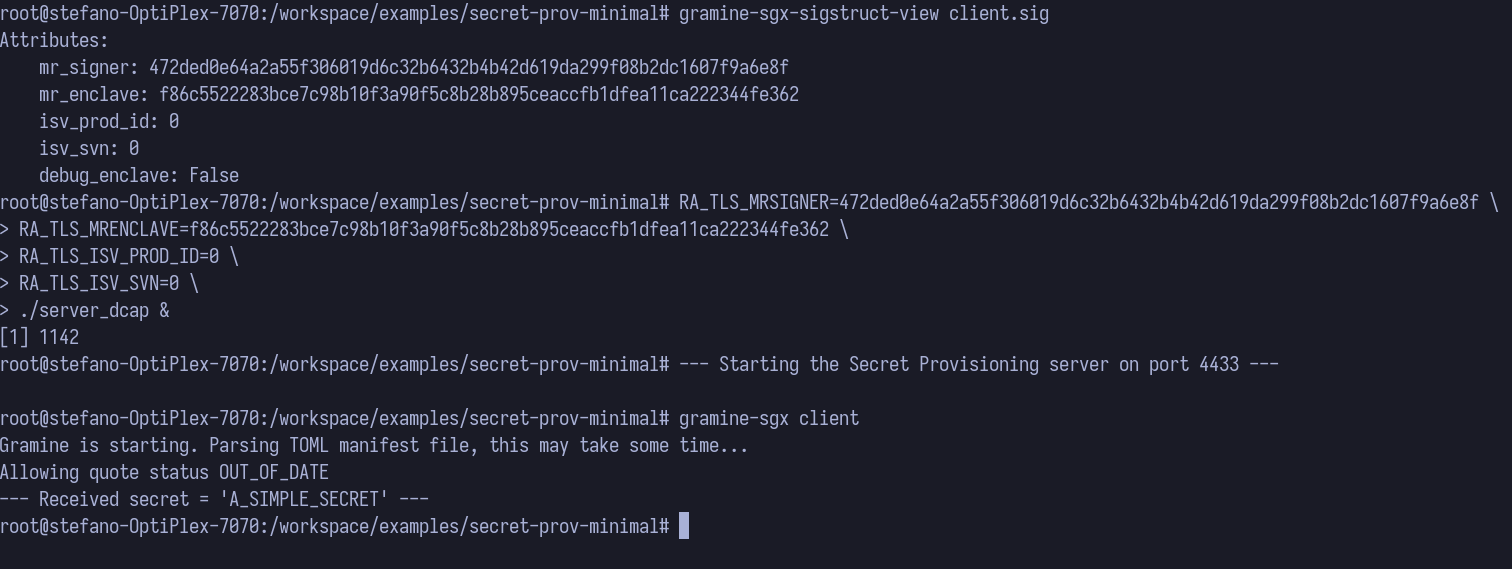
\includegraphics[width=0.95\textwidth]{figures/ch3/secret-prov-example.png}
  \end{center}
  \caption{Stampa dei parametri di firma dell'enclave, avvio del server e condivisione di un segreto statico}\label{fig:secret-prov-example}
\end{figure}

Il server può specificare una \textit{callback} per comunicare con il client per creare un protocollo più complicato. Come mostrato in \cref{lst:server-secret-prov-callback}, il server può interagire con il client attraverso \textit{secret\_provision\_write} e \textit{secret\_provision\_read}.

\begin{lstlisting}[language=c,caption=Interazione continua con il client,label=lst:server-secret-prov-callback]
static int communicate_with_client_callback(struct ra_tls_ctx* ctx) {
    int ret;

    /* if we reached this callback, the first secret was sent successfully */
    printf("--- Sent secret1 ---\n");

    /* let's send another secret (just to show communication with secret-awaiting client) */
    uint8_t buf[sizeof(EXPECTED_STRING)] = {0};

    ret = secret_provision_read(ctx, buf, sizeof(buf));
    if (ret < 0) {
        if (ret == -ECONNRESET) {
            /* client doesn't want another secret, shutdown communication gracefully */
            return 0;
        }

        fprintf(stderr, "[error] secret_provision_read() returned %d\n", ret);
        return -EINVAL;
    }

    if (memcmp(buf, EXPECTED_STRING, sizeof(EXPECTED_STRING))) {
        fprintf(stderr, "[error] client sent '%s' but expected '%s'\n", buf, EXPECTED_STRING);
        return -EINVAL;
    }

    ret = secret_provision_write(ctx, (uint8_t*)SECOND_SECRET, sizeof(SECOND_SECRET));
    if (ret < 0) {
        fprintf(stderr, "[error] secret_provision_write() returned %d\n", ret);
        return -EINVAL;
    }

    printf("--- Sent secret2 = '%s' ---\n", SECOND_SECRET);
    return 0;
}
int main(void) {
    puts("--- Starting the Secret Provisioning server on port " PORT " ---");
    ret = secret_provision_start_server((uint8_t*)FIRST_SECRET, sizeof(FIRST_SECRET),
                                        PORT, SRV_CRT_PATH, SRV_KEY_PATH,
                                        NULL,
                                        communicate_with_client_callback);
    if (ret < 0) {
        fprintf(stderr, "[error] secret_provision_start_server() returned %d\n", ret);
        return 1;
    }
    return 0;
} 
\end{lstlisting}

\subsection{Applicazione Data Sealing}
\subsubsection{Gramine}
Il sealing dei dati sul disco può essere fatto specificando \textbf{\textit{encrypted}} come valore dell'attributo \textit{type} di un \textit{mount}, come mostrato in \cref{lst:gramine-data-sealing}. Di conseguenza, tutti i file (ricorsivamente) saranno cifrati. La chiave con cui vengono cifrati i file può essere specificata in $3$ modi:
\begin{itemize}
  \item \textit{hardcoded}: per motivi di test e per rendere riproducibili gli esperimenti, una chiave può essere fornita come stringa esadecimale \cref{lst:gramine-data-sealing};
  \item \textit{unique}: usando i nomi \textit{\_sgx\_mrenclave} o \textit{\_sgx\_mrsigner} si utilizzano delle chiavi che rende impossibile decifrare i file su altre piattaforme SGX in quanto legate alla firma dell'enclave;
  \item \textit{shared}: recuperata da un servizio remoto con le API di secret provisioning
\end{itemize}

\begin{lstlisting}[language=toml,caption=Cartelle cifrate con differenti modalità,label=lst:gramine-data-sealing]
loader.env.LD_PRELOAD = "libsecret_prov_attest.so"
loader.env.SECRET_PROVISION_CONSTRUCTOR = "1"
loader.env.SECRET_PROVISION_SET_KEY = "test"
loader.env.SECRET_PROVISION_CA_CHAIN_PATH = "/ca.crt"
loader.env.SECRET_PROVISION_SERVERS = "localhost:4433"
sgx.remote_attestation = "dcap"
fs.mounts = [
  { type = "encrypted", path = "/db1/", uri = "file:db1/", key_name = "default" },
  { type = "encrypted", path = "/db2/", uri = "file:db2/", key_name = "_sgx_mrenclave" },
  { type = "encrypted", path = "/db3/", uri = "file:db3/", key_name = "test" },
]
fs.insecure__keys.default = "ffeeddccbbaa99887766554433221100"
\end{lstlisting}
L'applicazione scrive in $3$ cartelle differenti un messaggio e questo viene cifato secondo le modalità descritte sopra. 

\lstinputlisting[language=c,caption="Scrittura in 3 diversi file con altrettante modalità di cifratura"]{../gramine/examples/data-sealing/main.c}

Il secret provisioning viene effettuato utilizzando un server analogo a quello dell'esempio precedente, mentre di seguito viene riportato il manifest completo.

\lstinputlisting[language=Toml,caption="Manifest file che illustra le differenti modalità di fare data sealing"]{../gramine/examples/data-sealing/sealing.manifest.template}

L'applicazione può essere compilata come mostrato di seguito. Prima di eseguire l'enclave, bisogna eseguire il server con i parametri dell'enclave come mostrato in \cref{fig:secret-prov-example}.
\begin{verbatim}
make clean app build dcap 
\end{verbatim}

\subsubsection{OpenEnclave}
OpenEnclave non fornisce API di alto livello come quelle di gramine, ma mette a disposizione delle funzioni per fare il \textit{sealing} dei dati utilizzando una chiave \textit{unique} ricavata in modo simile all'enclave. La specifica EDL in \cref{lst:edl-data-seal-example}, definisce due funzioni (\textbf{\textit{seal\_data}} e \textbf{\textit{unseal\_data}}) che cifrano un buffer di dati nell'enclave a partire da una privacy policy che può essere:
\begin{itemize}
  \item \textit{unique}: i dati sono accessibili sono dall'enclave che l'ha cifrata;
  \item \textit{product}: i dati possono essere decifrati da tutti le enclave che eseguono sulla piattaforma;
\end{itemize}

\lstinputlisting[caption=File EDL per applicazione data sealing,label=lst:edl-data-seal-example]{../openenclave/examples/data-sealing/datasealing.edl}
Queste due funzioni, utilizzano le primitive di openenclave \textit{oe\_seal} e \textit{oe\_unseal} per cifrare i dati configurando automaticamente le chiavi. Ad esempio, in \cref{lst:oe-seal-data-example}, è riportato come viene implementata la \textit{oe\_seal}.

\begin{lstlisting}[language=c,caption=Utilizzo di oe\_seal,label=lst:oe-seal-data-example]
 
int ecall_dispatcher::seal_data(
    int seal_policy,
    const unsigned char* optional_message,
    size_t optional_message_size,
    const unsigned char* data,
    size_t data_size,
    data_t* sealed_data)
{
    oe_result_t ret;
    uint8_t* blob;
    size_t blob_size;
    sealed_data_t* temp_sealed_data;

    if (optional_message_size > sizeof(temp_sealed_data->optional_message))
        return OE_INVALID_PARAMETER;

    const oe_seal_setting_t settings[] = {OE_SEAL_SET_POLICY(seal_policy)};
    ret = oe_seal(
        NULL,
        settings,
        sizeof(settings) / sizeof(*settings),
        data,
        data_size,
        optional_message,
        optional_message_size,
        &blob,
        &blob_size);
    if (ret != OE_OK)
    {
        TRACE_ENCLAVE("oe_seal() failed with %d\n", ret);
        goto exit;
    }
    if (blob_size > UINT32_MAX)
    {
        TRACE_ENCLAVE("blob_size is too large to fit into an unsigned int");
        ret = OE_OUT_OF_MEMORY;
        goto exit;
    }

    temp_sealed_data =
        (sealed_data_t*)malloc(sizeof(*temp_sealed_data) + blob_size);
    if (temp_sealed_data == NULL)
    {
        ret = OE_OUT_OF_MEMORY;
        goto exit;
    }

    memset(temp_sealed_data, 0, sizeof(*temp_sealed_data));
    memcpy(
        temp_sealed_data->optional_message,
        optional_message,
        optional_message_size);
    temp_sealed_data->sealed_blob_size = blob_size;
    memcpy(temp_sealed_data + 1, blob, blob_size);

    sealed_data->data = (uint8_t*)temp_sealed_data;
    sealed_data->size = sizeof(*temp_sealed_data) + blob_size;

exit:
    oe_free(blob);
    return (int)ret;
}
\end{lstlisting}

Dall'host vengono fatte delle ECALL per cifrare dei dati che poi vengono salvati su file e poi decifrati. Una parte del codice è riportata in \cref{lst:host-data-sealing}. 

\begin{lstlisting}[language=c,caption=Codice host che effettua il sealing e unsealing dei dati,label=lst:host-data-sealing]
enclave = create_enclave(argv[1]);
data = (unsigned char*)g_plain_text;
data_size = strlen((const char*)data) + 1;
result = seal_data(
  enclave,
  &ret,
  policy,
  (unsigned char*)g_opt_msg,
  strlen(g_opt_msg),
  data,
  data_size,
  &sealed_data);
// Save sealed data to file
sealed_file.open("sealed", ios::out | ios::binary);
sealed_file.write(reinterpret_cast<const char*>(sealed_data.data), sealed_data.size);
sealed_file.close();
cout << "Host: Sealed data saved to file 'sealed'" << endl;

// read from file and decrypt
result = unseal_data(enclave, &ret, &sealed_data, 1, &unsealed_data);

// print unsealed data
cout << "Host: Unsealed result:" << endl;
printf("data=%s --- ", unsealed_data.data);

printf("data_size=%zd\n", unsealed_data.size);
\end{lstlisting}

Il programma può essere compilato ed eseguito con il comando di seguito. Il risultato è riportato in \cref{fig:oe-seal-data-example}.
\begin{verbatim}
make clean private.pem all run
\end{verbatim}

\begin{figure}
  \begin{center}
    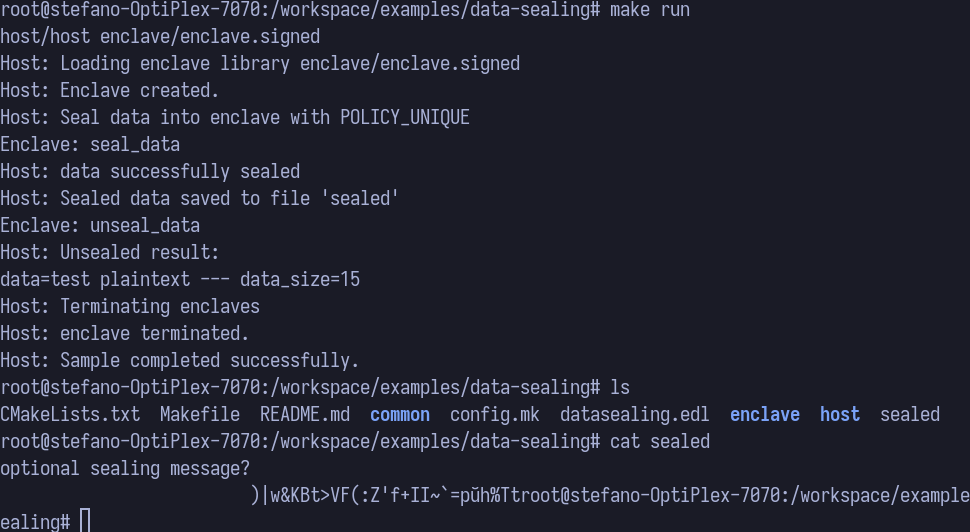
\includegraphics[width=0.95\textwidth]{figures/ch3/oe-data-sealing-example.png}
  \end{center}
  \caption{Esecuzione del programma e ispezione del file sealed}\label{fig:oe-seal-data-example}
\end{figure}

\clearpage
\section{Sviluppi futuri: Intel Trusted Domains Extentions (TDX)}
Lo sviluppo di SGX ha subito un rallentamento in favore di tecnologie che sfruttano la virtualizzazione. Intel nel 2021 ha proposto \textbf{\textit{Trusted Domain Extensions } (TDX)} che introduce un'altra modalità all'interno della CPU: \textbf{\textit{Secure Arbitration Mode (SEAM)}} (\cref{fig:tdx-architecture}). TDX è un'implementazione di TEE basata su macchine virtuali come \textit{CoVE} e AMD-SEV.

Intel TDX mette insieme diverse tecnologie consolidate per offrire un'implementazione TEE con supporto per la virtualizzazione\cite{Cheng2024} quali:
\begin{itemize}
  \item Intel VT-x: tecnologia che supporta la virtualizzazione in hardware unitamente a EPT;
  \item Intel SGX: implementazione di TEE in \textit{user space};
  \item Intel MKTME/TME: tecnologia per cifrare la memoria con diverse chiavi il cui identificativo viene codificato nei bit più alti dell'indirizzo;
\end{itemize}

\begin{figure}[h]
  \begin{center}
    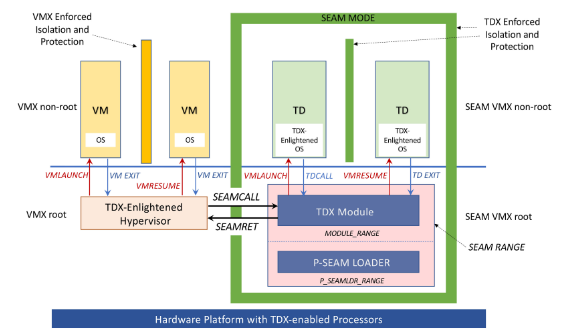
\includegraphics[width=.65\textwidth]{figures/tdx-architecture.png}
  \end{center}
  \caption{Architettura di TDX}\label{fig:tdx-architecture}
\end{figure}

\subsection{Virtualizzazione}
Il concetto principale di TDX è il \textbf{\textit{Trusted Domain} (TD)} di cui viene garantita la confidenzialità e l'integrità della memoria e dello stato delle vCPU. TDX utilizza VT per garantire la separazione i \textit{trusted domains}. In particolare, il modulo TDX e i TD eseguono in un nuovo stato all'interno degli stati \textit{VMX Root} e \textit{Non root}. Nelle prime versioni di TDX non è disponibile la virtualizzazione innestata e c'è un limitato supporto alla condivisione di memoria. Per ogni TD, sono create due EPT: una privata e cifrata e un'altra in chiaro.
\subsection{Memory protection}
La protezione della memoria viene fatta utilizzando la \textbf{\textit{Multiple Keys Total Memory Encryption} (MKTME)}. La cifratura della memoria viene affidata completamente al modulo TDX che gestisce le chiavi di ogni singolo TD. MKTME prevede la cifratura della memoria con una chiave identificata da un \textbf{\textit{Host Key Identifier} (HKID)} codificata all'interno dell'indirizzo fisico e memorizzata in una tabella detta \textbf{\textit{Key Encryption Table} (KET)}. Lo spazio delle chiavi è diviso in:
\begin{itemize}
  \item HKID private: chiavi assegnate a singoli TD;
  \item HKID shared: chiavi utilizzate per la memoria condivisa;
\end{itemize}
\subsection{Attestazione}
In TDX, l'attestazione è fortemente collegata alle \textit{architectural enclaves} presentate in precedenza. TDX effettua un'attestazione locale con la Quoting Enclave e utilizza i servizi spiegati in precedenza per effettuare l'attestazione DCAP come in SGX. Il Quote di TDX include un certificato rilasciato da Intel.

\clearpage
\pagestyle{plain}
\pagenumbering{roman}
\setcounter{page}{1}
\addcontentsline{toc}{section}{Riferimenti}
\bibliographystyle{plain}
\bibliography{refs}

\end{document}
